\section{TransNet V2}\label{sec:transnetv2}

The original TransNet network, as described in the previous section, has a set of limitations. In this section, we discuss them in detail and propose changes to mitigate them. In the next section, we thoroughly evaluate and discuss the proposed solutions. The contributions in this Section are presented in paper \cite{soucek2020transnetv2}.

\subsection{Limitations of TransNet}\label{sec:limitsoftransnet}
Shots for TransNet training are created artificially without taking into account their real distribution in the wild, aside from focusing on the most prevalent types of transitions. Even though it is convenient, automatically constructing training samples has multiple downsides. Commonly, in the real videos, subsequent shots share the same scene only captured from a different angle by another camera or at a different time. These shots can have very similar features such as color histograms, which makes them impossible to detect by such simple features. In TransNet training, as shots are concatenated randomly, the concatenated shots often do not share semantic meaning across the shots -- the shots can be completely arbitrary -- which does not force the network to learn more advanced features needed for difficult transitions in the real distribution. Another problem is the selection of the segments/shots. In the case of the IACC.3 dataset, they are detected automatically by a shot detection algorithm, which itself has false negatives and false positives. The false negatives do not present a challenge since they are scarce, and the probability of sampling undetected transitions is low as the actual shots are usually many seconds long. However, false positives in high dynamic scenes mean that such hard negatives are missing in the dataset. Since the dynamic scenes are probably the hardest for any detection algorithm, it may be needed to manually label at least some dynamic scenes and use them as hard negatives. This approach was taken, for example, by Hassanien et al. Finally, the last problem is that the artificially created dataset contains only a fixed set of selected transition types. However, not many types of transitions are commonly used, so this does not present a big problem.

% - train data. however convenient, automatically constructing training samples has multiple downsides - the dataset contains only contains the selected types of transitions selected by author (which is probably not a big deal since not many types of transitions are used in the wild). as the shots are concatenated randomly, the concatenated shots often do not share semantic meaning across shots - the shots can by completely arbitrary which makes it easier task that it is actually in the wild. we need the segments to join - these need to be selected automatically eg. by trivial shot detection algorithm - that means the segments contain transitions undetected by the detection algorithm - which in general is not a problem since it occurs not often since actual shots are usually dozen seconds long so the probability of sampling undetected transitions is low. however the bigger problem is that highly dynamic scenes - that are actually caused by sparse sampling of an action eg. 30fps - they are probably the hardest for any detection algorithm - they are split in multiple shots and we do not see them in our dataset as hard negatives. ----- with clipshots larger native dataset however worse?? - presented in the end of the chapter

The datasets used for TransNet validation and testing are very limited in size as well as very limited in transition types presented in the data. Also, the validation dataset is created by a single person without any peer review or independent verification, and the videos themselves contain mostly user-generated content of poor quality that no longer reflects the current state of user-generated videos. Nowadays, many cell phones contain high-resolution cameras with high dynamic range (HDR) support and image stabilization. HDR suppresses over-exposures and under-exposures that commonly resulted in false positives. Optical image stabilization and advanced digital stabilization \cite{PixelStabilization} reduces handshake very prevalent in content from older devices. Further, professional video equipment that produces even less of such artifacts is becoming ubiquitous in amateur video production. Our validation and test sets should also reflect that.

%- validation and test data. Rai dataset used for testing is very limited in size as well very limited in transitions presented in the data. our validation dataset is created by single person without any pier review or independent verification. the data themselves contain mostly user generated content with poor quality with no longer reflect the state of user generated content now with modern cell phone cameras with crisp high resolution content with high dynamic range and suppressed over exposures and underexposures that commonly resulted into false positives. also optical image stabilization and advanced digital stabilization \cite{google digital stabilization in Google Pixel} reduces hand shakes very common in content from older device. cinematic content contains unusually even less of such artefacts. Our validation and test sets should also reflect that.


With the automatically precisely generated transitions without any compression and resizing artifacts, we see rapid over-fitting even already after a few hundred batches, and the technique of early stopping needs to be employed. That means the model is not trained until convergence, but only until the performance on the validation set stops improving. While training the model further improves loss and performance on the synthetically generated datasets, it harms performance on the real data. To mitigate the over-fitting, there have been developed many techniques such as L2 regularization or dropout \cite{dropout}. These techniques impose restrictions preventing the model from being stuck in bad local minima and forcing the model to focus on all activation values instead of only a small discriminative set that is sensitive to noise.

Another approach to over-fitting is to vary input data to make models robust to such changes. In the image domain, there have been developed many techniques for data augmentation revolving around contrast, color or brightness changes, input masking \cite{cutout}, and others. Recently, even reinforcement algorithms were used to create the best augmentation methods for a certain task \cite{autoaugment}. In our work, however, it is necessary to augment not only video frames but also the transition generation process itself. Such augmentation is unique to shot boundary detection task, and not much work has been done in this area since only a handful of works use automatically generated datasets. We discuss our solutions for the input data generation and augmentation in the next paragraphs.


% There have been developed multiple ways to mitigate the over-fitting. Some methods intentionally force the model not to focus only on certain features and not to rely on certain small set of weights (rewrite) such as dropout, L2 regularization (as MAP?), batch normalization.. On the other hand over fitting can be mitigated by data augmentation - the input data is varied in order to make the network robust to such changes. In image domain these often revolve around contrast, brightness changes, changes in color - such as saturation and hue. in recent years reinforcement algorithms were used to create the best augmentation methods for certain task and certain datasets \cite{autoaugment}. we however also need to augment the transition themselves, such augmentation is unique to shot boundary detection task and not much work has been done towards it since only handful of works use automatically generated datasets.


\subsection{Datasets and Data Augmentation}\label{sec:transnetv2DatasetsAugm}
Unlike Hassanien et al. \cite{Hassanien17}, we refrain from a fixed pre-generated dataset, which enables us to employ various types of augmentation. We also utilize recently published large manually annotated shot boundary dataset ClipShots. We describe the dataset and augmentation methods, including their technical details, in this Section.


\subsubsection{Large Dataset}
With the introduction of ClipShots \cite{Tang2018}, a dataset purposefully collected for shot boundary detection, we no longer have to rely on automatic transition generation since the dataset contains 166,756 manually annotated transitions. Hard cuts consist of 77 percent of the dataset, while the rest is gradual transitions, including dissolves and wipes. For training, we extract 160 frames long segments, each with a transition in the middle, then during training, a randomly cropped segment of length $N=100$ is used. This way we ensure each training segment contains a transition. We assume hard negatives are contained in these segments, and we do not explicitly train the network on sequences without any transition.

However, as reported in the results section, interestingly, training only on real data does not achieve the best performance. We therefore also utilize both IACC.3 and ClipShot datasets for automatic transition generation. Note the manual annotation of ClipShots does not have the problem of false positives in dynamic scenes, as discussed in Section \ref{sec:limitsoftransnet}; therefore, we could also benefit from that fact compared to training only on IACC.3. For the train set, we extract 300 frames long segments from each scene from the start, the middle, and the end of the scene while skipping some, if the scene is shorter. For scenes shorter than 300 frames, we store the whole scene. During training, we select two random segments and randomly crop them to the length of 100 frames and join them by a random transition at a random position. If a segment is shorter than 100 frames and the position of the transition means the final transition sample would be shorter than 100 frames, the sample is discarded and not used for training.

Aside from our original IACC.3 100 video validation set, we use 457 videos from the official ClipShots train set for validation. For testing the official ClipShots test set \cite{Tang2018}, BBC Planet Earth documentary series \cite{BaraldiScenes} and RAI \cite{Baraldi15} datasets are used. Again only predictions for 50 middle frames from the whole 100 frame input sequence are used to eliminate errors due to limited context.

\subsubsection{Shot Augmentation}
We apply standard image augmentation to each shot with all images in the shot being augmented the same way in order not to create random color changes in a single shot. When generating transition artificially, we augment the shot prior to the shot joining. Firstly shot frames are flipped left to right with probability $0.5$ and top to bottom with probability $0.1$. Further, standard TensorFlow image operations adjusting saturation, contrast, brightness, and hue are utilized. Saturation and contrast of a shot are changed by a random factor from range $\left[0.8,1.2\right]$. Brightness and hue are changed by random delta from range $\left[-0.1,0.1\right]$. We also use \textit{Equalize}, \textit{Posterize} and \textit{Color} operations from Python image library PIL\footnote{\url{https://pillow.readthedocs.io}, re-implemented in TensorFlow at \url{https://github.com/tensorflow/tpu/blob/master/models/official/efficientnet/autoaugment.py}.}. Each operation is applied with probability $0.05$, \textit{Posterize} randomly keeps four to seven bits of the original color, \textit{Color} is applied with random factor from range $\left[0.5,1.5\right]$.

\begin{figure}[b]
    \centering
    \newcolumntype{C}[1]{>{\centering\arraybackslash}p{#1}}
    \begin{tabular}{cC{0.7cm}cC{0.7cm}c}
    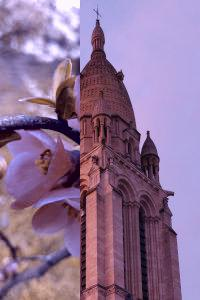
\includegraphics[align=c,width=.2\textwidth]{img/transnetv2/noslide.jpg}
    &
    &
    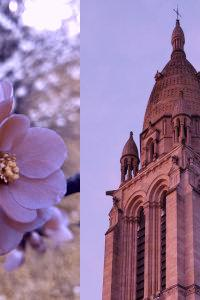
\includegraphics[align=c,width=.2\textwidth]{img/transnetv2/slide_both.jpg}
    &
    &
    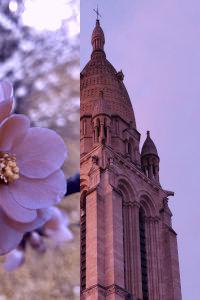
\includegraphics[align=c,width=.2\textwidth]{img/transnetv2/slide_one.jpg}
    \end{tabular}
    \caption[Examples of additional transition types]{Examples of additional transition types. Standard wipe (left), flower scene sliding in while church scene sliding out (middle) and flower scene sliding in while church scene stationary (right).}
    \label{fig:types_of_wipe}
\end{figure}
\subsubsection{Transition Types}
Similarly to the original TransNet, we generate hard cuts and dissolves. We generate 50\% of hard cuts and 50\% of dissolves, the length of each dissolve is randomly uniformly selected from the set of even lengths $\{2,4,\dots, 28, 30\}$. We generate only even lengths of dissolve transitions so that the ground truth position of the transition is exactly defined (for each frame we predict whether there is a transition from the current frame to the next frame, i.e. in case of odd lengths the transition can be either to the left or to the right of the middle frame).

As the ClipShots test set contains also wipes, we experiment with adding wipes into possible transition types. In 5\% of dissolves, we generate wipe instead of the dissolve. We consider both horizontal and vertical wipes. We also consider sliding in the entering scene, sliding out the exiting scene, or both. See Figure \ref{fig:types_of_wipe} for illustrations of different types of wipes. However, we observe no improvement in performance with wipes in the train set; therefore, we refrain from generating them.

\subsubsection{Color Transfer}
To force the network to learn more advanced local features instead of simple global features, we introduce shot color augmentation technique we call color transfer. Given two shots we transfer color from one shot $s_1$ to the other shot $s_2$ by first transforming both shots to CIE Lab color space, then we compute the new shot $s_2'$ by the following equation:
\begin{equation*}
    s_2' = \frac{\sigma_1}{\sigma_2} (s_2 - \hat{s}_2) + \hat{s}_1
\end{equation*}
where $\hat{s}_i$ is mean and $\sigma_i$ standard deviation of pixel values for respective shots. The equation is applied pixel-wise on each of the three Lab channels independently. Finally, we transform the new shot back to RGB color space. An example of the color transfer can be seen in Figure \ref{fig:color_transfer}. During training, the color transfer is applied randomly to 10\% of generated input sequences.


\begin{figure}[h]
    \centering
    \newcolumntype{C}[1]{>{\centering\arraybackslash}p{#1}}
    \begin{tabular}{cC{0.7cm}cC{0.7cm}c}
    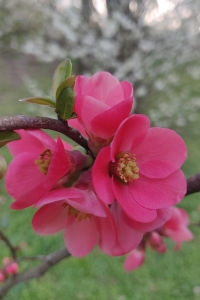
\includegraphics[align=c,width=.2\textwidth]{img/transnetv2/IMG_20190404_180509_edited.jpg}
    &
    $+$
    &
    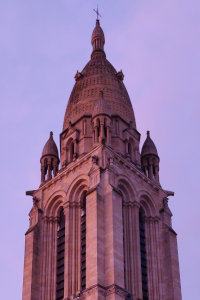
\includegraphics[align=c,width=.2\textwidth]{img/transnetv2/IMG_20200307_191029_edited.jpg}
    &
    $\rightarrow$
    &
    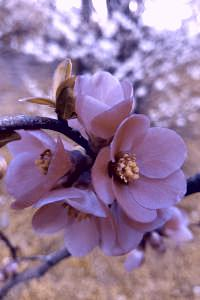
\includegraphics[align=c,width=.2\textwidth]{img/transnetv2/IMG_20190404_180509_transfered.jpg}
    \end{tabular}
    \caption[Color transfer augmentation technique between two shots]{Example of color transfer augmentation technique between two shots.}
    \label{fig:color_transfer}
\end{figure}

\subsubsection{Suppressing False Positives}
We consider adding two types of special augmentation to reduce false positives caused by handshake and rapid change of illumination e.g. by a passing object in front of a light source. Handshake is applied to five percent of train sequences by randomly removing the top (or bottom) $k\in\{1, \dots, 5\}$ pixels from the first $m$ frames and removing bottom (or top respectively) $k$ pixels from the subsequent $N-m$ frames. Finally, the frames are bilinearly resized to their original shape. Illumination change is applied to five percent of train sequences by performing the standard shot augmentation to only part of the sequence.

As the RAI dataset contains multiple sequences where color is changed between two subsequent frames, the illumination augmentation slightly improves the results. However, the opposite is seen on ClipShots and BBC datasets, where the addition of this type of augmentation creates more false negatives than it creates true negatives since these phenomena are not prevalent in these test sets.
Therefore in the final model training, we use neither artificial illumination changes nor handshake augmentation. Also, further manual inspection reveals the network can learn to suppress flashes purely from unaugmented data (Figure \ref{fig:transnetv2_predicted_transitions}A).




\subsection{Architecture Improvements}
Our TransNet V2 is based on the original TransNet network with three SDDCNN blocks, each with two DDCNN cells. However, we make a wide range of changes that substantially improve the network's performance. A schema of the TransNet V2 network is shown in Figure \ref{fig:nn_architecture_v2}, and all the changes are described in detail in the following paragraphs.

\begin{figure}
    \centering
    \begin{tikzpicture}[
    font=\sffamily\scriptsize,
    box/.style={
    	draw,
    	minimum width=0.7cm,
    	minimum height=0.4cm,
    	rounded corners=2, inner sep=2pt, align=center, anchor=north,
    	text width=1.7cm
    }, pil/.style={
    	-{Stealth[scale=.5]},
    	rounded corners=2pt,
    	line width=1pt
    }, pil2/.style={
    	rounded corners=2pt,
    	line width=1pt
    }]
    \definecolor{my-green}{RGB}{208, 240, 192}
    \definecolor{my-yellow}{RGB}{247, 231, 206}
    \definecolor{my-blue}{RGB}{195, 236, 255}
    \definecolor{my-red}{RGB}{247, 183, 183}
    
    \node[box, draw=none, text width=1cm] (input) at (0,3.3) {Input};
    \node[box, fill=my-red] (colorhist) at (2.5,-6.6) {RGB hist.\\similarities};
    \draw[pil2] (input) |- (1.5, 2.75);
    \draw[pil] (1.5, 2.75) -| (colorhist);
    
    
    \node[box, fill=my-green, text width=3cm] (layer1a) at (0,2.5) {DDCNN V2 cell\\[-2pt]{\tiny 64 filters}};
    \node[box, fill=my-green, text width=3cm] (layer1b) at (1.7,1.6) {DDCNN V2 cell\\[-2pt]{\tiny 64 filters}};
    \node[draw, circle, inner sep=1pt, align=center, anchor=north] (add1) at (0,0.9) {\textbf{+}};
    \node[box, anchor=north, fill=my-yellow] (avg-pool1) at (0,0.2) {Avg pooling\\1$\times$2$\times$2};
    
    \path[pil] (input) edge node[anchor=east] {\tiny\textit{N$\times$48$\times$27$\times$3}} (layer1a);
    \draw[pil2] (layer1a) |- (1, 1.8);
    \draw[pil] (1, 1.8) -| (layer1b);
    \draw[pil] (layer1a) -- (add1);
    \draw[pil] (layer1b) |- (add1);
    \path[pil] (add1) edge node[anchor=west] {\tiny\textit{N$\times$48$\times$27$\times$64}} (avg-pool1);
    

    \node[box, fill=my-green, text width=3cm] (layer2a) at (0,-.9) {DDCNN V2 cell\\[-2pt]{\tiny 128 filters}};
    \node[box, fill=my-green, text width=3cm] (layer2b) at (1.7,-1.8) {DDCNN V2 cell\\[-2pt]{\tiny 128 filters}};
    \node[draw, circle, inner sep=1pt, align=center, anchor=north] (add2) at (0,-2.5) {\textbf{+}};
    \node[box, anchor=north, fill=my-yellow] (avg-pool2) at (0,-3.2) {Avg pooling\\1$\times$2$\times$2};
    
    \path[pil] (avg-pool1) edge node[anchor=west] {\tiny\textit{N$\times$24$\times$13$\times$64}} (layer2a);
    \draw[pil2] (layer2a) |- (1, -1.6);
    \draw[pil] (1, -1.6) -| (layer2b);
    \draw[pil] (layer2a) -- (add2);
    \draw[pil] (layer2b) |- (add2);
    \path[pil] (add2) edge node[anchor=west] {\tiny\textit{N$\times$24$\times$13$\times$128}} (avg-pool2);

    
    \node[box, fill=my-green, text width=3cm] (layer3a) at (0,-4.3) {DDCNN V2 cell\\[-2pt]{\tiny 256 filters}};
    \node[box, fill=my-green, text width=3cm] (layer3b) at (1.7,-5.2) {DDCNN V2 cell\\[-2pt]{\tiny 256 filters}};
    \node[draw, circle, inner sep=1pt, align=center, anchor=north] (add3) at (0,-5.9) {\textbf{+}};
    \node[box, anchor=north, fill=my-yellow] (avg-pool3) at (0,-6.6) {Avg pooling\\1$\times$2$\times$2};
    
    \path[pil] (avg-pool2) edge node[anchor=west] {\tiny\textit{N$\times$12$\times$6$\times$128}} (layer3a);
    \draw[pil2] (layer3a) |- (1, -5);
    \draw[pil] (1, -5) -| (layer3b);
    \draw[pil] (layer3a) -- (add3);
    \draw[pil] (layer3b) |- (add3);
    \path[pil] (add3) edge node[anchor=west] {\tiny\textit{N$\times$12$\times$6$\times$256}} (avg-pool3);
    
    
    \node[box, text width=1.2cm] (flatten) at (0,-7.7) {Flatten};
    \path[pil] (avg-pool3) edge node[anchor=west] {\tiny\textit{N$\times$6$\times$3$\times$256}} (flatten);
    
    \node[box, text width=1.2cm] (concat) at (0,-8.5) {Concat};
    \path[pil] (flatten) edge node[anchor=west] {\tiny\textit{N$\times$4608}} (concat);
    
    \path[pil2] (colorhist) edge node[anchor=east] {\tiny\textit{N$\times$128}} (2.5, -8.5);
    \draw[pil] (2.5, -8.5) |- (concat);

    \node[box, anchor=north, fill=my-red] (framesim) at (-2.5,-6.6) {Learnable\\similarities};
    
    \draw[pil2] (avg-pool1) |- (-1, -0.65);
    \draw[pil] (-1, -0.65) -| (-2.7,-6.6);
    \draw[pil2] (avg-pool2) |- (-1, -4.05);
    \draw[pil] (-1, -4.05) -| (-2.5,-6.6);
    \draw[pil2] (avg-pool3) |- (-1, -7.45);
    \draw[pil2] (-1, -7.45) -| (-1.25, -7);
    \draw[pil2] (-1.25, -7) |- (-1.5, -6.1);
    \draw[pil] (-1.5, -6.1) -| (-2.3, -6.6);
    
    \path[pil2] (framesim) edge node[anchor=west] {\tiny\textit{N$\times$128}} (-2.5, -8.5);
    \draw[pil] (-2.5, -8.5) |- (concat);
    
    \node[box, fill=my-blue, text width=2.2cm] (dense1) at (0,-9.3) {Dense + ReLU};
    \node[box] (dropout) at (0,-10.1) {Dropout\\[-2pt]{\tiny rate 0.5}};
    \node[box, fill=my-blue] (dense2) at (-1.4,-11) {Dense};
    \node[box] (sigmoid) at (-1.4,-11.8) {Sigmoid};
    \node[box, fill=my-blue] (dense2-multihead) at (1.4,-11) {Dense};
    \node[box] (sigmoid-multihead) at (1.4,-11.8) {Sigmoid};
    
    \path[pil] (concat) edge node[anchor=west] {\tiny\textit{N$\times$4864}} (dense1);
    \path[pil] (dense1) edge node[anchor=west] {\tiny\textit{N$\times$1024}} (dropout);
    \draw[pil2] (dropout) |- (-1,-10.8);
    \draw[pil] (-1,-10.8) -| (dense2);
    \draw[pil2] (dropout) |- (1,-10.8);
    \draw[pil] (1,-10.8) -| (dense2-multihead);
    \path[pil] (dense2) edge node[anchor=west] {\tiny\textit{N$\times$1}} (sigmoid);
    \path[pil] (dense2-multihead) edge node[anchor=west] {\tiny\textit{N$\times$1}} (sigmoid-multihead);
    
    \draw[decorate,decoration={brace}] (-2.4,-12.2) -- (-2.4,-11) node[midway, anchor=center,sloped, above=0.1, font=\sffamily\tiny, align=center] {Single transition\\frame prediction};
    \draw[decorate,decoration={brace}] (2.4,-11) -- (2.4,-12.2) node[midway, anchor=center,sloped, above=0.1, font=\sffamily\tiny, align=center] {All transition\\frames prediction};

    %
    %
    
    \end{tikzpicture}
    \caption[TransNet V2 shot boundary detection network architecture]{TransNet V2 shot boundary detection network architecture. Note that $N$ represents the length of a video sequence, not batch size.}
    \label{fig:nn_architecture_v2}
\end{figure}


\subsubsection{Convolution Kernel Factorization}
The TransNet benefits from using four decoupled convolutions instead of a single one since the decoupling reduces the number of parameters and the network is less prone to over-fitting, and also speeds up the computation. We further investigate how to factorize the convolution kernel to reduce over-fitting while preserving the benefits of a large field of view. In the image domain, depthwise separable convolutions have been introduced. The depthwise spatial convolution acts on each input channel separately and is followed by a pointwise (the standard $1\times 1$) convolution, which combines the resulting output channels. This way, the network is limited to learn only factorizable kernels; however, Chollet \cite{Chollet_2017_CVPR} shows it improves classification performance of InceptionV3 network \cite{Szegedy_2016_InceptionV3} on ImageNet \cite{imagenet}.

In video domain, Xie et al. \cite{Xie_2018_ECCV} disentangles 3D $k \times k \times k$ convolutions into 2D $k\times k$ spatial convolution and 1D temporal convolution with kernel size $k$ to improve I3D's \cite{Carreira_2017_CVPR} performance on multiple datasets. Practically the separable 3D convolution can be implemented by two standard 3D convolutions with kernel shapes $1 \times k \times k$ for the spatial and $k \times 1 \times 1$ for the temporal convolution. This factorization of the convolutional kernel forces the network to learn to extract image features in the first step and to compare them temporarily in the second step. It also potentially reduces number of trainable parameters -- $N_{in}\times k^2\times F$ for the spatial kernel and $F\times k\times N_{out}$ for the temporal kernel compared to standard $N_{in}\times k^3\times N_{out}$. If the number of input filters $N_{in}$ is the same as output filters $N_{out}$, then if the number of filters $F$ in between the spatial and temporal convolution is smaller than $N_{out}\cdot k^3 / (k^2 + k)$, the number of trainable parameters of the separable 3D convolution is lower than the number of parameters of the standard convolution. For kernel size $k=3$ we may select any $F < 2.25 N_{out}$ while still lowering the parameter count.

In our case, we observe that setting $F=N_{out}$ is too extreme parameter reduction, hampering the performance of the model. However, setting $F=2 N_{out}$ improves the performance substantially. Figure \ref{fig:ddcnnv2} shows the new version of the DDCNN block with factorized convolutions.

\begin{figure}
    \centering
    \begin{tikzpicture}[
    font=\sffamily\scriptsize,
    box/.style={
    	draw,
    	minimum width=0.7cm,
    	minimum height=0.4cm,
    	rounded corners=2, inner sep=2pt, align=center, anchor=north,
    	text width=1.7cm
    }, pil/.style={
    	-{Stealth[scale=.5]},
    	rounded corners=2pt,
    	line width=1pt
    }]
    \definecolor{my-green}{RGB}{208, 240, 192}
    \definecolor{my-yellow}{RGB}{247, 231, 206}
    \definecolor{my-blue}{RGB}{195, 236, 255}

    
    \node[box, draw=none, text width=1cm] (input) at (0,3) {Input};
    
    %%% DDCNN cell
    \node[box, fill=my-green] (layer1-1) at (-3,2) {Conv 1$\times$3$\times$3};
    \node[box, fill=my-green] (layer1-2) at (-1,2) {Conv 1$\times$3$\times$3};
    \node[box, fill=my-green] (layer1-3) at (1,2) {Conv 1$\times$3$\times$3};
    \node[box, fill=my-green] (layer1-4) at (3,2) {Conv 1$\times$3$\times$3};
    
    \node[box, fill=my-green] (layer2-1) at (-3,1.2) {Conv 3$\times$1$\times$1\\[-2pt]{\tiny dilation 1}};
    \node[box, fill=my-green] (layer2-2) at (-1,1.2) {Conv 3$\times$1$\times$1\\[-2pt]{\tiny dilation 2}};
    \node[box, fill=my-green] (layer2-3) at (1,1.2) {Conv 3$\times$1$\times$1\\[-2pt]{\tiny dilation 4}};
    \node[box, fill=my-green] (layer2-4) at (3,1.2) {Conv 3$\times$1$\times$1\\[-2pt]{\tiny dilation 8}};
    
    \node[box, text width=1.2cm] (layer-out) at (0,0.4) {Concat};
    
    \node[box, anchor=north, fill=my-yellow, text width=3cm] (bn) at (0,-0.4) {Batch Normalization};
    
    \node[box, text width=1.2cm] (relu) at (0,-1.) {ReLU};

    %%% EDGES
    \draw[rounded corners=2pt, line width=1pt] (input) |- (-0.3,2.3);
    \draw[rounded corners=2pt, line width=1pt] (input) |- (0.3,2.3);
    
    \draw[pil] (-0.3,2.3) -| (layer1-1);
    \draw[pil] (-0.3,2.3) -| (layer1-2);
    \draw[pil] (0.3,2.3) -| (layer1-3);
    \draw[pil] (0.3,2.3) -| (layer1-4);

    \draw[pil] (layer1-1) edge node[anchor=east] {\tiny 2F filters} (layer2-1);
    \draw[pil] (layer1-2) edge node[anchor=east] {\tiny 2F filters} (layer2-2);
    \draw[pil] (layer1-3) edge node[anchor=west] {\tiny 2F filters} (layer2-3);
    \draw[pil] (layer1-4) edge node[anchor=west] {\tiny 2F filters} (layer2-4);
    
    \draw[line width=1pt] (layer2-1) edge node[anchor=east,near end] {\tiny F filters} (-3, 0.32);
    \draw[line width=1pt] (layer2-2) edge node[anchor=east,near end] {\tiny F filters} (-1, 0.32);
    \draw[line width=1pt] (layer2-3) edge node[anchor=west,near end] {\tiny F filters} (1, 0.32);
    \draw[line width=1pt] (layer2-4) edge node[anchor=west,near end] {\tiny F filters} (3, 0.32);
    
    \draw[pil] (-3, 0.32) |- (layer-out);
    \draw[pil] (-1, 0.32) |- (layer-out);
    \draw[pil] (1, 0.32) |- (layer-out);
    \draw[pil] (3, 0.32) |- (layer-out);
    
    \draw[pil] (layer-out) edge node[anchor=west] {\tiny 4F filters} (bn);
    \draw[pil] (bn) -- (relu);
    

    \end{tikzpicture}
    \caption[DDCNN V2 cell with 4F filters]{DDCNN V2 cell with 4F filters.}
    \label{fig:ddcnnv2}
\end{figure}

\subsubsection{Frame Similarities as Features}
As already discussed in the related work section, many methods extract individual frame features and use them to compute similarity scores between consequent frames. The scores are then used as an input to a machine learning model such as SVM that predicts the likelihood of transition purely from the similarity scores. Similarly, we improve the performance of TransNet's final fully-connected classifier by enriching the convolutional features by frame similarities. We consider frame similarities computed both from handcrafted and learnable features. A simple RGB color histogram with $8^3=512$ bins is used for the handcrafted features. For the learnable features, we take outputs of all SDDCNN blocks. Those outputs of shape $N\times H_l \times W_l \times C_l$ are spatially averaged into vectors of shape $N \times C_l$ and vectors from different levels $l$ are concatenated thus every one of the $N$ frames is represented by vector $v_i$ of length $\sum_{l=0}^L C_l$. A single linear layer without activation function is applied to reduce the dimension of the vector $v_i$ to 128.

For each frame, we compute cosine similarities of its handcrafted or learned features with fifty frames preceding the frame and fifty frames following the frame. The similarities are transformed by a single fully connected layer with the ReLU activation function into 128-dimensional space and are concatenated with the convolutional features. If not all of the fifty preceding or following frames are available due to the limited length $N$ of the input sequence zeros are used instead. Figure \ref{fig:frame_sim} depicts such computation for the learned features.

\begin{figure}
    \centering
    \begin{tikzpicture}[
    font=\sffamily\scriptsize,
    box/.style={
    	draw,
    	minimum width=0.7cm,
    	minimum height=0.4cm,
    	rounded corners=2, inner sep=2pt, align=center, anchor=north,
    	text width=1.7cm
    }, pil/.style={
    	-{Stealth[scale=.5]},
    	rounded corners=2pt,
    	line width=1pt
    }, pil2/.style={
    	rounded corners=2pt,
    	line width=1pt
    }, table/.style={
        matrix of nodes,
        row sep=-\pgflinewidth,
        column sep=-\pgflinewidth,
        nodes={
            rectangle,
            draw=black,
            align=center,
            inner sep=0pt,
            minimum height=0.35cm,
            text width=0.35cm,
        },
        font=\sffamily\tiny,
        nodes in empty cells,
    }]
    \definecolor{my-gray}{RGB}{251, 251, 251}
    \definecolor{my-yellow}{RGB}{247, 231, 206}
    \definecolor{my-blue}{RGB}{195, 236, 255}
    \definecolor{my-red}{RGB}{247, 183, 183}
    \definecolor{my-green}{RGB}{208, 240, 192}

    
    \node[box, draw=none, text width=1cm] (input) at (0,3) {Inputs};
    
    %%% DDCNN cell
    \node[box, fill=my-yellow, text width=1.2cm] (avg1) at (-1.5,2) {Spatial\\average};
    \node[box, fill=my-yellow, text width=1.2cm] (avg2) at (0,2) {Spatial\\average};
    \node[box, fill=my-yellow, text width=1.2cm] (avg3) at (1.5,2) {Spatial\\average};
    
    \path[pil] (-1.5, 2.4) edge node[anchor=east] {\tiny\textit{N$\times$24$\times$13$\times$64}} (avg1);
    \path[pil] (-.4, 2.4) edge node[anchor=west] {\tiny\textit{N$\times$12$\times$6$\times$128}} (-.4,2);
    \path[pil] (1.5, 2.4) edge node[anchor=west] {\tiny\textit{N$\times$6$\times$3$\times$256}} (avg3);
    
    \node[box, text width=1.2cm] (concat) at (0,0.9) {Concat};
    \node[box, fill=my-blue] (dense1) at (0,0.1) {Dense};
    
    \node[box, draw=lightgray, text width=3.4cm, text height=1.9cm, fill=my-gray] at (0.35,-0.65) {};
    \node[rotate=90, text=gray] at (-1.2, -1.7) {Cosine Sim};
    \node[box, fill=my-yellow] (normalize) at (0,-0.7) {Normalize};
    \node[box] (transpose) at (1.1,-1.4) {Transpose};
    \node[box] (matmul) at (0,-1.9) {Matrix\\Multiplication};
    
    \node[box, text width=2.2cm, fill=my-red] (gather) at (0,-3) {Pad + Gather};
    \node[box, fill=my-blue, text width=2.2cm] (dense2) at (0,-3.8) {Dense + ReLU};
    
    \path[pil2] (avg1) edge node[anchor=east] {\tiny\textit{N$\times$64}} (-1.5, 0.9);
    \path[pil] (avg2) edge node[anchor=west] {\tiny\textit{N$\times$128}} (concat);
    \path[pil2] (avg3) edge node[anchor=west] {\tiny\textit{N$\times$256}} (1.5, 0.9);
    \draw[pil] (-1.5, 0.95) |- (concat);
    \draw[pil] (1.5, 0.95) |- (concat);
    
    \path[pil] (concat) edge node[anchor=west] {\tiny\textit{N$\times$448}} (dense1);
    \path[pil] (dense1) edge node[anchor=west] {\tiny\textit{N$\times$128}} (normalize);
    \path[pil] (matmul) edge node[anchor=west] {\tiny\textit{N$\times$N}} (gather);
    \path[pil] (gather) edge node[anchor=west] {\tiny\textit{N$\times$101}} (dense2);
    \path[pil] (dense2) edge node[anchor=west] {\tiny\textit{N$\times$128}} (0,-4.6);
    
    \draw[pil2] (normalize) |- (0.5, -1.2);
    \draw[pil] (0.5, -1.2) -| (transpose);
    
    \draw[pil] (transpose) |- (matmul);
    \draw[pil] (normalize) -- (matmul);
    

    \matrix (table1) [table] at (6,-0.1){
    |[fill=my-green!100]|1  & |[fill=my-green!70]|.8 & |[fill=my-green!35]|.6 & .6 & .4 \\
    |[fill=my-green!70]|.8 &  |[fill=my-green!100]|1 & |[fill=my-green!70]|.7 & |[fill=my-green!35]|.7 & .5 \\
    |[fill=my-green!35]|.6 & |[fill=my-green!70]|.7 &  |[fill=my-green!100]|1 & |[fill=my-green!70]|.9 & |[fill=my-green!35]|.6 \\
    .6 & |[fill=my-green!35]|.7 & |[fill=my-green!70]|.9 &  |[fill=my-green!100]|1 & |[fill=my-green!70]|.7 \\
    .4 & .5 & |[fill=my-green!35]|.6 & |[fill=my-green!70]|.7 &  |[fill=my-green!100]|1 \\
    };
    
    \node[box, text width=2.2cm, fill=my-red, anchor=center] (gather2) at (6,-1.5) {Pad + Gather};
    
    \matrix (table2) [table] at (6,-2.9){
    0  &  0 & |[fill=my-green!100]|1  & |[fill=my-green!70]|.8 & |[fill=my-green!35]|.6 \\
    0  & |[fill=my-green!70]|.8 & |[fill=my-green!100]|1  & |[fill=my-green!70]|.7 & |[fill=my-green!35]|.7 \\
    |[fill=my-green!35]|.6 & |[fill=my-green!70]|.7 & |[fill=my-green!100]|1  & |[fill=my-green!70]|.9 & |[fill=my-green!35]|.6 \\
    |[fill=my-green!35]|.7 & |[fill=my-green!70]|.9 & |[fill=my-green!100]|1  & |[fill=my-green!70]|.7 & 0  \\
    |[fill=my-green!35]|.6 & |[fill=my-green!70]|.7 & |[fill=my-green!100]|1  & 0  & 0  \\
    };

    \path[pil] (6, -0.98) edge (gather2);
    \path[pil] (gather2) edge (6, -2.02);

    \end{tikzpicture}
    \caption[Learnable frame similarities computation with visualization of Pad + Gather operation]{Learnable frame similarities computation with visualization of Pad + Gather operation (right).}
    \label{fig:frame_sim}
\end{figure}

\subsubsection{Shortcuts}
Some transitions are easy to detect by simple differencing in a minimal number of layers, others need the full depth of the network to be detected. We add a residual connection in each Stacked DDCNN block from the output of the first DDCNN cell in the block to the input of the spatial pooling operation.% Intuitively we think of the residual connections as short paths for easy transitions.

\subsubsection{Batch Normalization}
Neural network training is dependent on the initialization of the network's parameters. If parameters are not initialized carefully, activations inside the network can rise to extreme values, which in turn can result in getting stuck in poor local minima. We employ batch normalization technique \cite{BatchNormalization} that normalizes outputs of each layer by mean and variance computed from the input batch. It allows us to worry less about the learning rate and be less careful about parameter initialization. More importantly, it also acts as a regularizer, so the network is less prone to over-fitting.

\subsubsection{Multiple Classification Heads}
The original TransNet predicts every transition as a single frame transition, no matter the length. This representation has its benefit that (almost) every frame belongs to a scene -- no frames are `inside' a transition. Further, if two transitions are very close to each other, there is no ambiguity if it is a single long transition or two separate transitions. However, this representation does not provide information on transition length. Therefore we add a second prediction head that predicts all in-transition frames instead of only the middle one. 
In some of our preliminary experiments adding the second head slightly improves performance. We hypothesize the network can learn more easily what constitutes as a transition and how long the transition is. Note that even though the information on the length of a transition is readily available, we do not use it in any way in the evaluation phase. However, we believe utilizing this information could, for example, eliminate many double detections when a single long transition is detected multiple times.


\subsection{Other Changes}

\subsubsection{Optimizer}
In recent years there have been countless efforts to improve the standard stochastic gradient descent optimization method. RMSProp \cite{tieleman2012lecture} and Adam \cite{Adam14} have become some of the most widely adopted optimizers with both utilizing estimates of gradients' second moments. However, many state-of-the-art works in the image domain \cite{autoaugment, EfficientNet} refrain from using them and instead use rather primitive stochastic gradient descent with momentum while achieving better results. In our task, we observe that Adam optimizer is more effective in minimizing the loss than SGD with momentum; however, we see performance improvements on validation and test sets when using SGD with momentum compared to Adam.

\subsubsection{Regularization}
Artificially generated training data distribution is inherently different from the real data distribution. To reduce generalization error, we restrict the model's parameter space by also minimizing the square of $L_2$ norm of the parameters. Such action increases error on artificially generated validation data; however, it greatly reduces error on real data. Given the work of Loshchilov et al. \cite{FixingWeightDecay}, we also investigate whether decoupling the $L_2$ regularization from optimizer step computation -- a technique known as weight decay -- affects model's performance. While $L_2$ regularization and weight decay are (after hyper-parameter re-scaling) equivalent in the case of vanilla SGD, in more advanced optimizers, gradient moments estimations are affected by the square of $L_2$ norm of parameters in the loss. Loshchilov et al. argue this phenomenon is responsible for the inferior performance of Adam. However, in our case, when using SGD with momentum, we do not see any significant difference between $L_2$ regularization and weight decay.

Another form of regularization we employ is Dropout \cite{dropout}. It addresses the over-fitting problem by randomly dropping units from the neural network during training. In TransNet V2, we drop activations of the first fully-connected layer with a probability $0.5$.

\subsubsection{Class Imbalance}
The main classification head of the network is trained with only one frame labeled as transition and the other frames as no transition. In the case of long dissolve transitions, missing the middle transition frame even by a single position results in a large penalty; therefore, the network is inclined not to predict these transitions with high confidence at all. The original TransNet solves the problem by adjusting the decision threshold to $0.1$. We look at the problem more generally and weight the positive class by $\gamma$. Based on the exact task and dataset at hand, we may increase or decrease $\gamma$ to increase recall or precision respectively. For example, in retrieval, 100\% recall is crucial, whereas high precision may be preferred elsewhere. %in commercial shot detection applications as false positives are right in front of user's eyes wheres undetected transition will likely remain undiscovered by the user therefore not damaging user's satisfaction with the product {\color{red} TODO - to bych asi netvrdil}.
In our experiments, $\gamma = 5$ is used.

\subsubsection{Loss Function}
To train both classification heads we use the standard cross entropy loss (Equation~\ref{eq:transnetv2_cross_entropy}) with sequence predictions $\hat{y}$, sequence ground truth $y$ and possibly a weight $w$ of the positive \textit{is-a-transition} class. Since we predict likelihood of a transition for every frame in an input frame sequence $\bm{x}$ of length $N$, the length of $\hat{y}$ and $y$ vectors is also $N$.
\begin{equation}
  \mathcal{L}(\hat{y}, y, w)=-\sum_{i=1}^{N} \big[ w y_i\log \hat{y}_i + (1-y_i)\log(1-\hat{y}_i) \big]
  \label{eq:transnetv2_cross_entropy}
\end{equation}
The joint objective is shown in Equation \ref{eq:transnetv2_loss}. The first term is the loss of the classification head $f^s$ predicting single transition frame for arbitrarily long transition, the second term is the loss of the classification head $f^a$ predicting all transition frames and is weighted by $\lambda_a=0.1$. These loss terms are averaged over the batch. Last term of the objective is $L_2$ regularization of model's parameters $\theta$ weighted by $\lambda_p=0.0001$.
\begin{equation}
    \min \frac{1}{|\mathcal{B}|} \sum_{\left(\bm{x},y^s,y^m\right)\in\mathcal{B}} \Big[ \mathcal{L}\big(f^s(\bm{x};\theta), y^s, \gamma\big) + \lambda_a \mathcal{L}\big(f^a(\bm{x};\theta), y^a, 1\big) \Big] + \frac{\lambda_p}{2} \sum_{\vartheta\in\theta}\|\vartheta\|^2_2 
    \label{eq:transnetv2_loss}
\end{equation}
In Figure \ref{fig:input_sample} we show a sample frame sequence $\bm{x}$ with both immediate and gradual transition and its two types of ground truth vectors $y^s$ and $y^a$ for the two classification heads. Note that artificially generated train frame sequences contain only a single transition per sequence; however, when training with real data, it is possible to have multiple transitions in a single frame sequence if the transitions are close to each other.

\begin{figure}
    \centering
    \begin{tikzpicture}[
    box/.style={
    	draw,
    	minimum width=1cm,
    	minimum height=0.6cm,
    	align=center,
    	anchor=center
    },
    element1/.style={
        draw,
        minimum width=0.4cm,
    	minimum height=0.4cm,
    	align=center,
    	anchor=center,
    	circle
    },
    element2/.style={
        draw,
    	inner sep=2.8pt,
    	align=center,
    	anchor=center,
    	diamond
    }]
    \definecolor{g1}{RGB}{220, 220, 220}
    \definecolor{g2}{RGB}{180, 180, 180}
    \definecolor{g3}{RGB}{140, 140, 140}
    \definecolor{g4}{RGB}{70, 70, 70}

    \node[align=center,anchor=center] at (-2.,0) {$\bm{x}$};
    \node[align=center,anchor=center] at (-2.,-0.7) {$y^s$};
    \node[align=center,anchor=center] at (-2.,-1.3) {$y^a$};
    \node[align=center,anchor=center] at (-1.2,0) {$=$};
    \node[align=center,anchor=center] at (-1.2,-0.7) {$=$};
    \node[align=center,anchor=center] at (-1.2,-1.3) {$=$};
   
    \node[align=center,anchor=center] at (0,-0.7) {$0$};
    \node[align=center,anchor=center] at (1.2,-0.7) {$0$};
    \node[align=center,anchor=center] at (2.4,-0.7) {$1$};
    \node[align=center,anchor=center] at (3.6,-0.7) {$0$};
    \node[align=center,anchor=center] at (4.8,-0.7) {$0$};
    \node[align=center,anchor=center] at (6,-0.7) {$0$};
    \node[align=center,anchor=center] at (7.2,-0.7) {$1$};
    \node[align=center,anchor=center] at (8.4,-0.7) {$0$};
    
    \node[align=center,anchor=center] at (0,-1.3) {$0$};
    \node[align=center,anchor=center] at (1.2,-1.3) {$1$};
    \node[align=center,anchor=center] at (2.4,-1.3) {$1$};
    \node[align=center,anchor=center] at (3.6,-1.3) {$1$};
    \node[align=center,anchor=center] at (4.8,-1.3) {$1$};
    \node[align=center,anchor=center] at (6,-1.3) {$0$};
    \node[align=center,anchor=center] at (7.2,-1.3) {$1$};
    \node[align=center,anchor=center] at (8.4,-1.3) {$0$};
    
    \node[box] (img1) at (0,0) {};
    \node[box] (img2) at (1.2,0) {};
    \node[box] (img3) at (2.4,0) {};
    \node[box] (img4) at (3.6,0) {};
    \node[box] (img5) at (4.8,0) {};
    \node[box] (img6) at (6,0) {};
    \node[box] (img7) at (7.2,0) {};
    \node[box] (img8) at (8.4,0) {};
    
    \node[element1] at (img1) {};
    \node[element1, g4] at (img2) {};
    \node[element1, g3] at (img3) {};
    \node[element1, g2] at (img4) {};
    \node[element1, g1] at (img5) {};
    \node[element1] at (img8) {};


    \node[element2, g1] at (img2) {};
    \node[element2, g2] at (img3) {};
    \node[element2, g3] at (img4) {};
    \node[element2, g4] at (img5) {};
    \node[element2] at (img6) {};
    \node[element2] at (img7) {};

    \end{tikzpicture}
    \caption[Frame sequence with its ground truth]{Frame sequence with its two types of ground truth.}
    \label{fig:input_sample}
\end{figure}




\clearpage
\section{Experiments}\label{sec:transnetv2_evaluation}
In this section, we describe in detail the training process of the TransNet V2 model. Further, we compare our model to related works, also detailing our reevaluation process for it. Lastly, an ablation study is made to justify our decisions in making TransNet V2.

\subsection{Training Details}
We initialize weights of all convolution operations by He normal initializer~\cite{He_2015_ICCV}. Fully connected layers are initialized by TensorFlow's default Glorot initiali\-zer~\cite{Xavier_Glorot_init}. Biases are initialized by zeros.
We optimize the loss function (Equation \ref{eq:transnetv2_loss}) by stochastic gradient descent with momentum set to $0.9$ and fixed learning rate~$0.01$.

The standard TransNet V2 model is trained only by artificially generated sequences from IACC.3 and ClipShots datasets as described in Section \ref{sec:transnetv2DatasetsAugm}. Fifty percent of transitions we generate are hard cuts and fifty percent are dissolves of max length 30 frames. Besides, we consider training TransNet V2 by 15\% of real transitions from the ClipsShots dataset, 35\% of automatically generated hard cuts, and 50\% of automatically generated dissolves. Input to the network is frame sequences of length $N=100$ with each frame of size 48$\times$27.

We train the network for 30 epochs, each with 750 batches of size 16. In case the network is trained also in part by real manually annotated transitions from the ClipShots dataset, we add 20 additional epochs, i.e. the network is trained in total by 600,000 transitions. Training by artificial data only longer than 30 epochs is unnecessary since the network then overfits. The best performing model on our ClipShots validation set is selected. Together with validation, the training takes approximately 17 hours on a single Tesla V100 16GB GPU. TensorFlow deep learning library has been used for all the experiments.

\subsection{Results}
We report results of TransNet V2 trained both with artificial data only and with 15\% of real data. Additionally, we report the results of the original TransNet retrained by our data generation pipeline (Section \ref{sec:transnetv2DatasetsAugm}). For each network we show mean F1 scores\footnote{The same evaluation metric as in Section \ref{sec:transnetV1Eval} is used. However, due to minor errors in ground truth of some test sets, we also count correctly any detection that misses ground truth by at most two frames. With correct ground truth its effect compared to the original metric is minimal.\label{fn:metric}} and their standard deviations on the test sets in Table \ref{tb:transnets_results}. The statistics are computed from three best epochs from each of three independent runs as measured on the ClipShots validation dataset. We see a clear dominance of TransNet V2, especially on the ClipShots dataset. Utilizing real transitions improves results on BBC Planet Earth dataset while it harms performance on ClipShots and especially on RAI. We further discuss this phenomenon of better results with artificially generated data compared to the real data in the next section.

\begin{table}[h]
	\centering
	\begin{tabular}{l@{\hspace{1cm}}cccc}
		\toprule
		\textbf{Model} & ClipShots & BBC  & RAI \\
		\midrule
		TransNet                             & $71.9 \pm 3.5$ & $94.0 \pm 0.6$ & $93.1 \pm 0.6$ \\
		TransNet V2                          & $\bm{77.5} \pm 0.3$ & $95.1 \pm 0.5$ & $\bm{93.2} \pm 0.9$ \\
		TransNet V2 (15\% real transitions)  & $77.0 \pm 0.8$ & $\bm{96.5} \pm 0.5$ & $91.2 \pm 1.1$ \\
		\bottomrule
	\end{tabular}
	\caption[Comparison of the original TransNet and TransNet V2]{Comparison of the original TransNet and TransNet V2. Mean F1 scores and standard deviations in percents. Computed from 9 model instances (3 best epochs of 3 independent runs as measured on ClipShots validation set).}
	\label{tb:transnets_results}
\end{table}

We compare TransNet V2 to related work in Table \ref{tb:transnet_related_work}. For TransNet models, we report the F1 score of the best model selected out of the nine instances based on its performance on the ClipShot validation set. To best of our knowledge, the best shot boundary detectors available, as reported by their authors, are DeepSBD by Hassanien et al., DSM by Tang et al., and our original TransNet. On RAI dataset these methods report F1 score 93.4\%, 93.5\%, and 94.3\% respectively. However, Hassanien et al. report results on neither ClipShots nor BBC dataset. Tang et al. report results on ClipShots but their validation method differs from our method\footref{fn:metric} described in Section \ref{sec:transnetV1Eval} and for example incorrectly counts double detection. Therefore we reevaluate both shot boundary detection models and report only these results. We discuss reevaluation details in Section \ref{sec:transnetv2Reevaluation}.

\begin{table}[h]
	\centering
	\sisetup{detect-weight=true,detect-inline-weight=math}
	\begin{tabular}{l@{\hspace{1cm}}S[table-format=2.1]S[table-format=2.1]S[table-format=2.1]}
		\toprule
		\textbf{Model} & \multicolumn{1}{c}{ClipShots} & \multicolumn{1}{c}{BBC}  & \multicolumn{1}{c}{RAI} \\
		\midrule
		TransNet                             & 74.8 & 94.6 & 93.4 \\
		TransNet V2                          & 77.5 & 95.8 & \bftabnum 94.4 \\
		TransNet V2 (15\% real transitions)  & \bftabnum 77.9 & \bftabnum 96.2 & 93.9 \\
		\midrule
		TransNet\textsuperscript{$\dagger$}        & 73.5 & 92.9 &  94.3 \\
        Hassanien et al. \cite{Hassanien17}             & 75.9\textsuperscript{$*$} & 92.6\textsuperscript{$*$} & 93.9\textsuperscript{$*$} \\
        Tang et al. \cite{Tang2018}, ResNet baseline & 76.1\textsuperscript{$*$} & 89.3\textsuperscript{$*$} & 92.8\textsuperscript{$*$} \\
		\bottomrule
		\multicolumn{4}{l}{\footnotesize \textsuperscript{$\dagger$} The original TransNet as reported in Chapter \ref{sec:transnetv1} and in \cite{soucek2019transnet}. Reevaluated.} \\
		\multicolumn{4}{l}{\footnotesize \textsuperscript{$*$} Our reevaluation with the best threshold. See Section \ref{sec:transnetv2Reevaluation} for more details.}  \\
	\end{tabular}
	\caption[Comparison of TransNet V2 with related work]{Comparison of TransNet V2 with related work. F1 scores in percents. In the case of TransNet entries, the model with the best F1 score on the validation set is shown.}
	\label{tb:transnet_related_work}
\end{table}


TransNet V2 clearly outperforms related work on both ClipShots and BBC Planet Earth datasets, on the latter almost halving the error achieved by the previous state-of-the-art. On the RAI dataset, all methods perform comparably. Relative low performance on ClipShots can be attributed to the fact that it contains multiple seemingly unannotated videos or video parts. Further, in many cases, a frame is annotated as a transition incorrectly. We show some interesting transitions with our predictions in Figure \ref{fig:transnetv2_predicted_transitions} to illustrate our model's strengths and weaknesses, in Figure \ref{fig:transnet_v1_v2_visualization_comparison} raw predictions are shown on a long video sequence comparing the original TransNet and TransNet V2. Here we list some of the main takeaways:
\begin{itemize}
    \item Many times the ground truth incorrectly labels flash as a transition; however, the model can correctly ignore it. Nonetheless, if there is an illumination change in multiple subsequent frames, the model struggles (Figure \ref{fig:transnetv2_predicted_transitions}A).
    \item Long transitions with custom animations or fade-ins with uncommon colors are usually missed by the model (Figure \ref{fig:transnetv2_predicted_transitions}B, only selected frames from the transition shown).
    \item It can happen that the model misses a transition that is easily distinguishable for humans. However, sometimes these transitions are missing in the ground truth data (Figure \ref{fig:transnetv2_predicted_transitions}C).
    \item The model struggles with heavy motion blur (Figure \ref{fig:transnetv2_predicted_transitions}D).
    \item Many times it is subjective whether there is a transition (Figure \ref{fig:transnetv2_predicted_transitions}E).
\end{itemize}
All in all, on ClipShots dataset the best instance of TransNet V2 achieves 5.7k true positives, 1.7k false positives, and 1.5k false negatives. This is in stark contrast to BBC Planet Earth dataset, where the model achieves almost six times as many false negatives as false positives (exactly 4537 true positives, 55 false positives, and 307 false negatives). Such discrepancy can be attributed to already mentioned missing annotations and many long, difficult, and sometimes ambiguous transitions in ClipShots dataset.

Concerning the RAI dataset, all models perform comparably with a slight exception of Tang et al. However, we refrain from making any conclusions as the dataset contains mainly TV shows with visual effects that account for possibly many ambiguities in the ground truth. For example, the frame sequence in Figure \ref{fig:ambiguous_sequence_rai} is contained with slight variations in the dataset more than 20 times, and classifying it as transitions can result in almost doubling the number of false positives achieved by our method.

\begin{figure}[h]
    \centering
    \begin{tikzpicture}

    \node[inner sep=0pt] at (-5.2,0)
    {
\includegraphics[width=2.4cm]{img/transnetv2/rai_scene/000.jpg}};
    \node[inner sep=0pt] at (-2.6,0)
    {
\includegraphics[width=2.4cm]{img/transnetv2/rai_scene/001.jpg}};
    \node[inner sep=0pt] at (0,0)
    {
\includegraphics[width=2.4cm]{img/transnetv2/rai_scene/002.jpg}};
    \node[inner sep=0pt] at (2.6,0)
    {
\includegraphics[width=2.4cm]{img/transnetv2/rai_scene/003.jpg}};
    \node[inner sep=0pt] at (5.2,0)
    {
\includegraphics[width=2.4cm]{img/transnetv2/rai_scene/004.jpg}};
    
    %\draw[-{to reversed[scale=.4]}, thick] (-6.4, -0.85) -- (-2.6, -0.85);
    %\draw[{to reversed[scale=.4]}-, thick] (0, -0.85) -- (6.4, -0.85);
    %\draw[dotted] (-6.4, -1) -- (6.4, -1);
    %\node at (0, -1.1) {};
    \end{tikzpicture}
    \caption[Ambiguous frame sequence from the RAI dataset]{Ambiguous frame sequence from the RAI dataset labeled as \textit{no-transition} in the ground truth data.}
    \label{fig:ambiguous_sequence_rai}
\end{figure}


There are many more ambiguities similar to Figure \ref{fig:ambiguous_sequence_rai}; therefore we conclude it is necessary to adjust the model's threshold or even training data to compensate for particularities of a task at hand in case the reader's definition of a transition differs from our train and test data. For that reason, we show precision-recall curves and F1 scores as a function of the model's threshold for our best model TransNet V2 trained with 15\% real transitions on all test sets (Figure \ref{fig:transnetv2_prcurve}).

\begin{figure}[h]
    \centering
    \definecolor{my-red}{RGB}{255,51,76}
    \definecolor{my-green}{RGB}{63,188,157}
    \definecolor{my-blue}{RGB}{25,116,210}
    
    \begin{tikzpicture}[/pgfplots/width=\linewidth, /pgfplots/height=\linewidth]
    \begin{axis}[% Axis labels
                 ymin=.6,ymax=1,xmin=0,xmax=1,
    			 % Axis labels
    			 table/col sep=comma,
        		 xlabel={Recall / Threshold},
        		 ylabel={Precision / F1},
         		 xlabel shift={-2pt},
        		 ylabel shift={-3pt},
         		 % General appearance
		         font=\small,
		         axis equal image=true,
		         enlargelimits=false,
		         clip=true,
		         nodes near coords, % Place nodes near each coordinate
		         point meta=explicit symbolic,
		         % Grids 
        	     grid style=dotted, grid=both,
                 major grid style={white!65!black},
        		 minor grid style={white!85!black},
		 		 xtick={0,0.1,...,1.1},
        		 ytick={0,0.1,...,1.1},
         		 minor xtick={0,0.02,...,1},
		         minor ytick={0,0.02,...,1},
        		 % Legend
        		 legend style={at={(0,0)},
                 		       anchor=south west}]
        
	\addlegendimage{/pgfplots/refstyle=plot:prplot,black}\addlegendentry{P/R curve}
    \addlegendimage{/pgfplots/refstyle=plot:f1plot,black}\addlegendentry{F1/Thr curve}
    \addlegendimage{my-green}\addlegendentry{ClipShots}
    \addlegendimage{my-blue}\addlegendentry{BBC}
    \addlegendimage{my-red}\addlegendentry{RAI}

    \addplot[my-green,mark size=1.7,thick,mark repeat=5, mark phase=5,mark=*,font=\scriptsize] table[x=Recall,y=Precision, meta index=0] {data/transnetv2-prcurve-clip.txt};\label{plot:prplot};
    \addplot[dashed,my-green,mark size=1.7,thick] table[x=Thr,y=F1] {data/transnetv2-prcurve-clip.txt};\label{plot:f1plot};

    \addplot[my-blue,mark size=1.7,thick,mark repeat=5, mark phase=5,mark=*,font=\scriptsize] table[x=Recall,y=Precision, meta index=0] {data/transnetv2-prcurve-bbc.txt};
    \addplot[dashed,my-blue,mark size=1.7,thick] table[x=Thr,y=F1] {data/transnetv2-prcurve-bbc.txt};

	% Human partitions leave-one-out evaluation
    \addplot[my-red,mark size=1.7,thick,mark repeat=5, mark phase=5,mark=*,font=\scriptsize] table[x=Recall,y=Precision, meta index=0] {data/transnetv2-prcurve-rai.txt};
    \addplot[dashed,my-red,mark size=1.7,thick] table[x=Thr,y=F1] {data/transnetv2-prcurve-rai.txt};

    \end{axis}
    \end{tikzpicture}
    
    \caption[Performance of the best TransNet V2 model]{Precision/Recall curve with corresponding thresholds next to the points (solid) and F1 score dependency on the threshold (dashed) for the best performing TransNet V2 model on all test sets.}
    \label{fig:transnetv2_prcurve}
\end{figure}



\begin{figure}
    \centering
    \begin{tikzpicture}
\definecolor{incorrect}{RGB}{255,51,76}
\definecolor{correct}{RGB}{63,188,157}

\node[inner sep=0pt] at (-7.8, 0) {A)};

\node[inner sep=0pt] at (-7.0, 0.52) {\scriptsize GT};
\node[fill=incorrect, inner sep=1.5pt] at (-7.0, 0.22) {\scriptsize NOK};

\node[inner sep=0pt] at (-7.0, -0.18) {\scriptsize Model};
\node[fill=correct, inner sep=1.5pt] at (-7.0, -0.48) {\scriptsize OK};

\node[inner sep=0pt] at (-5.2,0)
{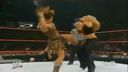
\includegraphics[width=2.4cm]{img/transnetv2/example_detections/0EXCdXUN_fk_001_07058.jpg}};
\node[inner sep=0pt] at (-2.6,0)
{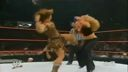
\includegraphics[width=2.4cm]{img/transnetv2/example_detections/0EXCdXUN_fk_001_07059.jpg}};
\node[inner sep=0pt] at (0,0)
{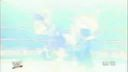
\includegraphics[width=2.4cm]{img/transnetv2/example_detections/0EXCdXUN_fk_001_07060.jpg}};
\node[inner sep=0pt] at (2.6,0)
{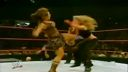
\includegraphics[width=2.4cm]{img/transnetv2/example_detections/0EXCdXUN_fk_001_07061.jpg}};
\node[inner sep=0pt] at (5.2,0)
{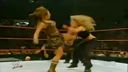
\includegraphics[width=2.4cm]{img/transnetv2/example_detections/0EXCdXUN_fk_001_07062.jpg}};

\draw[-{to reversed[scale=.4]}, thick] (-6.4, -0.85) -- (-2.6, -0.85);
\draw[{to reversed[scale=.4]}-, thick] (0, -0.85) -- (6.4, -0.85);

\draw[dotted] (-6.4, -1) -- (6.4, -1);

\node at (0, -1.1) {};
\end{tikzpicture}



\begin{tikzpicture}
\definecolor{incorrect}{RGB}{255,51,76}
\definecolor{correct}{RGB}{63,188,157}

\node[inner sep=0pt] at (-7.8, 0) {A)};

\node[inner sep=0pt] at (-7.0, 0.52) {\scriptsize GT};
\node[fill=incorrect, inner sep=1.5pt] at (-7.0, 0.22) {\scriptsize NOK};

\node[inner sep=0pt] at (-7.0, -0.18) {\scriptsize Model};
\node[fill=correct, inner sep=1.5pt] at (-7.0, -0.48) {\scriptsize OK};


\node[inner sep=0pt] at (-5.2,0)
{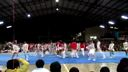
\includegraphics[width=2.4cm]{img/transnetv2/example_detections/Zoj_-rPnxGw_000_00144.jpg}};
\node[inner sep=0pt] at (-2.6,0)
{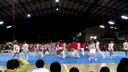
\includegraphics[width=2.4cm]{img/transnetv2/example_detections/Zoj_-rPnxGw_000_00145.jpg}};
\node[inner sep=0pt] at (0,0)
{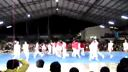
\includegraphics[width=2.4cm]{img/transnetv2/example_detections/Zoj_-rPnxGw_000_00146.jpg}};
\node[inner sep=0pt] at (2.6,0)
{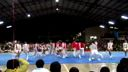
\includegraphics[width=2.4cm]{img/transnetv2/example_detections/Zoj_-rPnxGw_000_00147.jpg}};
\node[inner sep=0pt] at (5.2,0)
{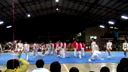
\includegraphics[width=2.4cm]{img/transnetv2/example_detections/Zoj_-rPnxGw_000_00148.jpg}};

\draw[-{to reversed[scale=.4]}, thick] (-6.4, -0.85) -- (-2.6, -0.85);
\draw[{to reversed[scale=.4]}-, thick] (0, -0.85) -- (6.4, -0.85);

\draw[dotted] (-6.4, -1) -- (6.4, -1);

\node at (0, -1.1) {};

\end{tikzpicture}

\begin{tikzpicture}
\definecolor{incorrect}{RGB}{255,51,76}
\definecolor{correct}{RGB}{63,188,157}

\node[inner sep=0pt] at (-7.8, 0) {A)};

\node[inner sep=0pt] at (-7.0, 0.52) {\scriptsize GT};
\node[fill=correct, inner sep=1.5pt] at (-7.0, 0.22) {\scriptsize OK};

\node[inner sep=0pt] at (-7.0, -0.18) {\scriptsize Model};
\node[fill=incorrect, inner sep=1.5pt] at (-7.0, -0.48) {\scriptsize NOK};



\node[inner sep=0pt] at (-5.2,0)
{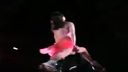
\includegraphics[width=2.4cm]{img/transnetv2/example_detections/7v_BpmoGuPI_000_02058.jpg}};
\node[inner sep=0pt] at (-2.6,0)
{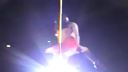
\includegraphics[width=2.4cm]{img/transnetv2/example_detections/7v_BpmoGuPI_000_02059.jpg}};
\node[inner sep=0pt] at (0,0)
{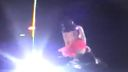
\includegraphics[width=2.4cm]{img/transnetv2/example_detections/7v_BpmoGuPI_000_02063.jpg}};
\node[inner sep=0pt] at (2.6,0)
{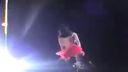
\includegraphics[width=2.4cm]{img/transnetv2/example_detections/7v_BpmoGuPI_000_02067.jpg}};
\node[inner sep=0pt] at (5.2,0)
{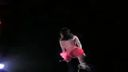
\includegraphics[width=2.4cm]{img/transnetv2/example_detections/7v_BpmoGuPI_000_02069.jpg}};

\draw[thick] (-6.4, -0.85) -- (6.4, -0.85);

\draw[dotted] (-6.4, -1) -- (6.4, -1);

\draw[line width=0.05cm] (-4.6, -1) -- (-3.2, -1);
\draw[line width=0.05cm] (4.6, -1) -- (3.2, -1);


\draw[] (-4.6, -0.92) -- (-4.6, -1.08);
\draw[] (-3.2, -0.92) -- (-3.2, -1.08);
\draw[] (4.6, -0.92) -- (4.6, -1.08);
\draw[] (3.2, -0.92) -- (3.2, -1.08);

\node at (0, -1.1) {};

\end{tikzpicture}


\begin{tikzpicture}
\definecolor{incorrect}{RGB}{255,51,76}
\definecolor{correct}{RGB}{63,188,157}

\node[inner sep=0pt] at (-7.8, 0) {B)};

\node[inner sep=0pt] at (-7.0, 0.52) {\scriptsize GT};
\node[fill=correct, inner sep=1.5pt] at (-7.0, 0.22) {\scriptsize OK};

\node[inner sep=0pt] at (-7.0, -0.18) {\scriptsize Model};
\node[fill=incorrect, inner sep=1.5pt] at (-7.0, -0.48) {\scriptsize NOK};


\node[inner sep=0pt] at (-5.2,0)
{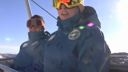
\includegraphics[width=2.4cm]{img/transnetv2/example_detections/-629gOGM1Ic_000_00286.jpg}};
\node[inner sep=0pt] at (-2.6,0)
{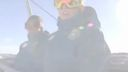
\includegraphics[width=2.4cm]{img/transnetv2/example_detections/-629gOGM1Ic_000_00289.jpg}};
\node[inner sep=0pt] at (0,0)
{
\includegraphics[width=2.4cm]{img/transnetv2/example_detections/-629gOGM1Ic_000_00291.jpg}};
\node[inner sep=0pt] at (2.6,0)
{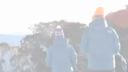
\includegraphics[width=2.4cm]{img/transnetv2/example_detections/-629gOGM1Ic_000_00294.jpg}};
\node[inner sep=0pt] at (5.2,0)
{
\includegraphics[width=2.4cm]{img/transnetv2/example_detections/-629gOGM1Ic_000_00296.jpg}};

\draw[-{to reversed[scale=.4]}, thick] (-6.4, -0.85) -- (-5.2, -0.85);
\draw[{to reversed[scale=.4]}-, thick] (5.2, -0.85) -- (6.4, -0.85);

\draw[dotted] (-6.4, -1) -- (6.4, -1);

\node at (0, -1.1) {};

\end{tikzpicture}


\begin{tikzpicture}
\definecolor{incorrect}{RGB}{255,51,76}
\definecolor{correct}{RGB}{63,188,157}

\node[inner sep=0pt] at (-7.8, 0) {B)};

\node[inner sep=0pt] at (-7.0, 0.52) {\scriptsize GT};
\node[fill=correct, inner sep=1.5pt] at (-7.0, 0.22) {\scriptsize OK};

\node[inner sep=0pt] at (-7.0, -0.18) {\scriptsize Model};
\node[fill=incorrect, inner sep=1.5pt] at (-7.0, -0.48) {\scriptsize NOK};



\node[inner sep=0pt] at (-5.2,0)
{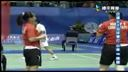
\includegraphics[width=2.4cm]{img/transnetv2/example_detections/5cUViKlaXS8_001_11719.jpg}};
\node[inner sep=0pt] at (-2.6,0)
{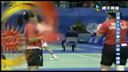
\includegraphics[width=2.4cm]{img/transnetv2/example_detections/5cUViKlaXS8_001_11723.jpg}};
\node[inner sep=0pt] at (0,0)
{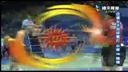
\includegraphics[width=2.4cm]{img/transnetv2/example_detections/5cUViKlaXS8_001_11730.jpg}};
\node[inner sep=0pt] at (2.6,0)
{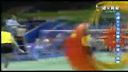
\includegraphics[width=2.4cm]{img/transnetv2/example_detections/5cUViKlaXS8_001_11740.jpg}};
\node[inner sep=0pt] at (5.2,0)
{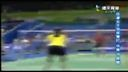
\includegraphics[width=2.4cm]{img/transnetv2/example_detections/5cUViKlaXS8_001_11745.jpg}};


\draw[-{to reversed[scale=.4]}, thick] (-6.4, -0.85) -- (-5.2, -0.85);
\draw[{to reversed[scale=.4]}-, thick] (5.2, -0.85) -- (6.4, -0.85);

\draw[dotted] (-6.4, -1) -- (6.4, -1);

\node at (0, -1.1) {};

\end{tikzpicture}

% \begin{tikzpicture}
% \definecolor{incorrect}{RGB}{255,51,76}
% \definecolor{correct}{RGB}{63,188,157}
% 
% 
% \node[inner sep=0pt] at (-7.0, 0.52) {\scriptsize GT};
% \node[fill=incorrect, inner sep=1.5pt] at (-7.0, 0.22) {\scriptsize NOK};
% 
% \node[inner sep=0pt] at (-7.0, -0.18) {\scriptsize Model};
% \node[fill=correct, inner sep=1.5pt] at (-7.0, -0.48) {\scriptsize OK};
% 
% \node[inner sep=0pt] at (-5.2,0)
% {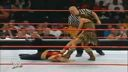
\includegraphics[width=2.4cm]{img/transnetv2/example_detections/0EXCdXUN_fk_000_06299.jpg}};
% \node[inner sep=0pt] at (-2.6,0)
% {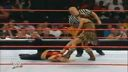
\includegraphics[width=2.4cm]{img/transnetv2/example_detections/0EXCdXUN_fk_000_06300.jpg}};
% \node[inner sep=0pt] at (0,0)
% {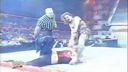
\includegraphics[width=2.4cm]{img/transnetv2/example_detections/0EXCdXUN_fk_000_06301.jpg}};
% \node[inner sep=0pt] at (2.6,0)
% {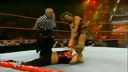
\includegraphics[width=2.4cm]{img/transnetv2/example_detections/0EXCdXUN_fk_000_06302.jpg}};
% \node[inner sep=0pt] at (5.2,0)
% {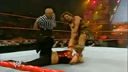
\includegraphics[width=2.4cm]{img/transnetv2/example_detections/0EXCdXUN_fk_000_06303.jpg}};
% 
% \draw[thick] (-6.4, -0.85) -- (6.4, -0.85);
% 
% \draw[dotted] (-6.4, -1) -- (6.4, -1);
% 
% \draw[line width=0.05cm] (0.6, -1) -- (2, -1);
% 
% \draw[] (0.6, -0.92) -- (0.6, -1.08);
% \draw[] (2, -0.92) -- (2, -1.08);
% 
% \node at (0, -1.1) {};
% \end{tikzpicture}

    

\begin{tikzpicture}
\definecolor{incorrect}{RGB}{255,51,76}
\definecolor{correct}{RGB}{63,188,157}

\node[inner sep=0pt] at (-7.8, 0) {C)};

\node[inner sep=0pt] at (-7.0, 0.52) {\scriptsize GT};
\node[fill=incorrect, inner sep=1.5pt] at (-7.0, 0.22) {\scriptsize NOK};

\node[inner sep=0pt] at (-7.0, -0.18) {\scriptsize Model};
\node[fill=correct, inner sep=1.5pt] at (-7.0, -0.48) {\scriptsize OK};


\node[inner sep=0pt] at (-5.2,0)
{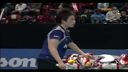
\includegraphics[width=2.4cm]{img/transnetv2/example_detections/1qAzo9Gdw1k_001_00965.jpg}};
\node[inner sep=0pt] at (-2.6,0)
{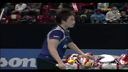
\includegraphics[width=2.4cm]{img/transnetv2/example_detections/1qAzo9Gdw1k_001_00966.jpg}};
\node[inner sep=0pt] at (0,0)
{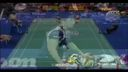
\includegraphics[width=2.4cm]{img/transnetv2/example_detections/1qAzo9Gdw1k_001_00967.jpg}};
\node[inner sep=0pt] at (2.6,0)
{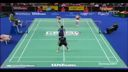
\includegraphics[width=2.4cm]{img/transnetv2/example_detections/1qAzo9Gdw1k_001_00968.jpg}};
\node[inner sep=0pt] at (5.2,0)
{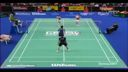
\includegraphics[width=2.4cm]{img/transnetv2/example_detections/1qAzo9Gdw1k_001_00969.jpg}};

\draw[thick] (-6.4, -0.85) -- (6.4, -0.85);

\draw[dotted] (-6.4, -1) -- (6.4, -1);

\draw[line width=0.05cm] (0.6, -1) -- (2, -1);

\draw[] (0.6, -0.92) -- (0.6, -1.08);
\draw[] (2, -0.92) -- (2, -1.08);

\node at (0, -1.1) {};

\end{tikzpicture}
    

% \begin{tikzpicture}
% \definecolor{incorrect}{RGB}{255,51,76}
% \definecolor{correct}{RGB}{63,188,157}
% 
% 
% \node[inner sep=0pt] at (-7.0, 0.52) {\scriptsize GT};
% \node[fill=incorrect, inner sep=1.5pt] at (-7.0, 0.22) {\scriptsize NOK};
% 
% \node[inner sep=0pt] at (-7.0, -0.18) {\scriptsize Model};
% \node[fill=correct, inner sep=1.5pt] at (-7.0, -0.48) {\scriptsize OK};
% 
% 
% \node[inner sep=0pt] at (-5.2,0)
% {
\includegraphics[width=2.4cm]{img/transnetv2/example_detections/1qAzo9Gdw1k_000_00084.jpg}};
% \node[inner sep=0pt] at (-2.6,0)
% {
\includegraphics[width=2.4cm]{img/transnetv2/example_detections/1qAzo9Gdw1k_000_00085.jpg}};
% \node[inner sep=0pt] at (0,0)
% {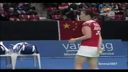
\includegraphics[width=2.4cm]{img/transnetv2/example_detections/1qAzo9Gdw1k_000_00086.jpg}};
% \node[inner sep=0pt] at (2.6,0)
% {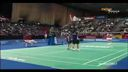
\includegraphics[width=2.4cm]{img/transnetv2/example_detections/1qAzo9Gdw1k_000_00087.jpg}};
% \node[inner sep=0pt] at (5.2,0)
% {\includegraphics[width=2.4cm]{img/transnetv2/example_detections/1qAzo9Gdw1k_000_00088.jpg}};
% 
% \draw[thick] (-6.4, -0.85) -- (6.4, -0.85);
% 
% \draw[dotted] (-6.4, -1) -- (6.4, -1);
% 
% \draw[line width=0.05cm] (0.6, -1) -- (2, -1);
% 
% \draw[] (0.6, -0.92) -- (0.6, -1.08);
% \draw[] (2, -0.92) -- (2, -1.08);
% 
% \node at (0, -1.1) {};
% \end{tikzpicture}
    

    

\begin{tikzpicture}
\definecolor{incorrect}{RGB}{255,51,76}
\definecolor{correct}{RGB}{63,188,157}

\node[inner sep=0pt] at (-7.8, 0) {C)};

\node[inner sep=0pt] at (-7.0, 0.52) {\scriptsize GT};
\node[fill=correct, inner sep=1.5pt] at (-7.0, 0.22) {\scriptsize OK};

\node[inner sep=0pt] at (-7.0, -0.18) {\scriptsize Model};
\node[fill=incorrect, inner sep=1.5pt] at (-7.0, -0.48) {\scriptsize NOK};



\node[inner sep=0pt] at (-5.2,0)
{\includegraphics[width=2.4cm]{img/transnetv2/example_detections/5cUViKlaXS8_000_02242.jpg}};
\node[inner sep=0pt] at (-2.6,0)
{\includegraphics[width=2.4cm]{img/transnetv2/example_detections/5cUViKlaXS8_000_02244.jpg}};
\node[inner sep=0pt] at (0,0)
{\includegraphics[width=2.4cm]{img/transnetv2/example_detections/5cUViKlaXS8_000_02245.jpg}};
\node[inner sep=0pt] at (2.6,0)
{\includegraphics[width=2.4cm]{img/transnetv2/example_detections/5cUViKlaXS8_000_02246.jpg}};
\node[inner sep=0pt] at (5.2,0)
{\includegraphics[width=2.4cm]{img/transnetv2/example_detections/5cUViKlaXS8_000_02248.jpg}};

\draw[-{to reversed[scale=.4]}, thick] (-6.4, -0.85) -- (-2.6, -0.85);
\draw[{to reversed[scale=.4]}-, thick] (2.6, -0.85) -- (6.4, -0.85);

\draw[dotted] (-6.4, -1) -- (6.4, -1);

\node at (0, -1.1) {};

\end{tikzpicture}

% \begin{tikzpicture}
% \definecolor{incorrect}{RGB}{255,51,76}
% \definecolor{correct}{RGB}{63,188,157}
% 
% 
% \node[inner sep=0pt] at (-7.0, 0.52) {\scriptsize GT};
% \node[fill=incorrect, inner sep=1.5pt] at (-7.0, 0.22) {\scriptsize NOK};
% 
% \node[inner sep=0pt] at (-7.0, -0.18) {\scriptsize Model};
% \node[fill=correct, inner sep=1.5pt] at (-7.0, -0.48) {\scriptsize OK};
% 
% \node[inner sep=0pt] at (-5.2,0)
% {\includegraphics[width=2.4cm]{img/transnetv2/example_detections/0nZQWIxsLB8_000_01417.jpg}};
% \node[inner sep=0pt] at (-2.6,0)
% {\includegraphics[width=2.4cm]{img/transnetv2/example_detections/0nZQWIxsLB8_000_01418.jpg}};
% \node[inner sep=0pt] at (0,0)
% {\includegraphics[width=2.4cm]{img/transnetv2/example_detections/0nZQWIxsLB8_000_01419.jpg}};
% \node[inner sep=0pt] at (2.6,0)
% {\includegraphics[width=2.4cm]{img/transnetv2/example_detections/0nZQWIxsLB8_000_01420.jpg}};
% \node[inner sep=0pt] at (5.2,0)
% {\includegraphics[width=2.4cm]{img/transnetv2/example_detections/0nZQWIxsLB8_000_01421.jpg}};
% 
% \draw[thick] (-6.4, -0.85) -- (6.4, -0.85);
% 
% \draw[dotted] (-6.4, -1) -- (6.4, -1);
% 
% \draw[line width=0.05cm] (0.6, -1) -- (2, -1);
% 
% \draw[] (0.6, -0.92) -- (0.6, -1.08);
% \draw[] (2, -0.92) -- (2, -1.08);
% 
% \node at (0, -1.1) {};
% 
% \end{tikzpicture}

\begin{tikzpicture}
\definecolor{incorrect}{RGB}{255,51,76}
\definecolor{correct}{RGB}{63,188,157}

\node[inner sep=0pt] at (-7.8, 0) {D)};

\node[inner sep=0pt] at (-7.0, 0.52) {\scriptsize GT};
\node[fill=correct, inner sep=1.5pt] at (-7.0, 0.22) {\scriptsize OK};

\node[inner sep=0pt] at (-7.0, -0.18) {\scriptsize Model};
\node[fill=incorrect, inner sep=1.5pt] at (-7.0, -0.48) {\scriptsize NOK};


\node[inner sep=0pt] at (-5.2,0)
{\includegraphics[width=2.4cm]{img/transnetv2/example_detections/0kzuXD0PmNg_000_06005.jpg}};
\node[inner sep=0pt] at (-2.6,0)
{\includegraphics[width=2.4cm]{img/transnetv2/example_detections/0kzuXD0PmNg_000_06006.jpg}};
\node[inner sep=0pt] at (0,0)
{\includegraphics[width=2.4cm]{img/transnetv2/example_detections/0kzuXD0PmNg_000_06007.jpg}};
\node[inner sep=0pt] at (2.6,0)
{\includegraphics[width=2.4cm]{img/transnetv2/example_detections/0kzuXD0PmNg_000_06008.jpg}};
\node[inner sep=0pt] at (5.2,0)
{\includegraphics[width=2.4cm]{img/transnetv2/example_detections/0kzuXD0PmNg_000_06009.jpg}};

\draw[thick] (-6.4, -0.85) -- (6.4, -0.85);

\draw[dotted] (-6.4, -1) -- (6.4, -1);

\draw[line width=0.05cm] (-0.6, -1) -- (-2, -1);

\draw[] (-0.6, -0.92) -- (-0.6, -1.08);
\draw[] (-2, -0.92) -- (-2, -1.08);

\node at (0, -1.1) {};

\end{tikzpicture}

    

\begin{tikzpicture}
\definecolor{incorrect}{RGB}{255,51,76}
\definecolor{correct}{RGB}{63,188,157}

\node[inner sep=0pt] at (-7.8, 0) {D)};

\node[inner sep=0pt] at (-7.0, 0.52) {\scriptsize GT};
\node[fill=correct, inner sep=1.5pt] at (-7.0, 0.22) {\scriptsize OK};

\node[inner sep=0pt] at (-7.0, -0.18) {\scriptsize Model};
\node[fill=incorrect, inner sep=1.5pt] at (-7.0, -0.48) {\scriptsize NOK};



\node[inner sep=0pt] at (-5.2,0)
{\includegraphics[width=2.4cm]{img/transnetv2/example_detections/-17hVQk3wXI_000_03859.jpg}};
\node[inner sep=0pt] at (-2.6,0)
{\includegraphics[width=2.4cm]{img/transnetv2/example_detections/-17hVQk3wXI_000_03861.jpg}};
\node[inner sep=0pt] at (0,0)
{\includegraphics[width=2.4cm]{img/transnetv2/example_detections/-17hVQk3wXI_000_03862.jpg}};
\node[inner sep=0pt] at (2.6,0)
{\includegraphics[width=2.4cm]{img/transnetv2/example_detections/-17hVQk3wXI_000_03863.jpg}};
\node[inner sep=0pt] at (5.2,0)
{\includegraphics[width=2.4cm]{img/transnetv2/example_detections/-17hVQk3wXI_000_03864.jpg}};

\draw[thick] (-6.4, -0.85) -- (6.4, -0.85);

\draw[dotted] (-6.4, -1) -- (6.4, -1);

\draw[line width=0.05cm] (0.6, -1) -- (2, -1);

\draw[] (0.6, -0.92) -- (0.6, -1.08);
\draw[] (2, -0.92) -- (2, -1.08);

\node at (0, -1.1) {};

\end{tikzpicture}
    
    

\begin{tikzpicture}
\definecolor{incorrect}{RGB}{255,51,76}
\definecolor{correct}{RGB}{63,188,157}
\definecolor{unknown}{RGB}{180,180,180}

\node[inner sep=0pt] at (-7.8, 0) {E)};

\node[inner sep=0pt] at (-7.0, 0.52) {\scriptsize GT};
\node[fill=unknown, inner sep=1.5pt] at (-7.0, 0.22) {\scriptsize ??};

\node[inner sep=0pt] at (-7.0, -0.18) {\scriptsize Model};
\node[fill=unknown, inner sep=1.5pt] at (-7.0, -0.48) {\scriptsize ??};


\node[inner sep=0pt] at (-5.2,0)
{\includegraphics[width=2.4cm]{img/transnetv2/example_detections/6e2-G6CXeT0_000_01253.jpg}};
\node[inner sep=0pt] at (-2.6,0)
{\includegraphics[width=2.4cm]{img/transnetv2/example_detections/6e2-G6CXeT0_000_01254.jpg}};
\node[inner sep=0pt] at (0,0)
{\includegraphics[width=2.4cm]{img/transnetv2/example_detections/6e2-G6CXeT0_000_01255.jpg}};
\node[inner sep=0pt] at (2.6,0)
{\includegraphics[width=2.4cm]{img/transnetv2/example_detections/6e2-G6CXeT0_000_01256.jpg}};
\node[inner sep=0pt] at (5.2,0)
{\includegraphics[width=2.4cm]{img/transnetv2/example_detections/6e2-G6CXeT0_000_01257.jpg}};

\draw[thick] (-6.4, -0.85) -- (6.4, -0.85);

\draw[dotted] (-6.4, -1) -- (6.4, -1);

\draw[line width=0.05cm] (0.6, -1) -- (2, -1);

\draw[] (0.6, -0.92) -- (0.6, -1.08);
\draw[] (2, -0.92) -- (2, -1.08);

\node at (0, -1.1) {};

\end{tikzpicture}

    

\begin{tikzpicture}
\definecolor{incorrect}{RGB}{255,51,76}
\definecolor{correct}{RGB}{63,188,157}
\definecolor{unknown}{RGB}{180,180,180}

\node[inner sep=0pt] at (-7.8, 0) {E)};

\node[inner sep=0pt] at (-7.0, 0.52) {\scriptsize GT};
\node[fill=unknown, inner sep=1.5pt] at (-7.0, 0.22) {\scriptsize ??};

\node[inner sep=0pt] at (-7.0, -0.18) {\scriptsize Model};
\node[fill=unknown, inner sep=1.5pt] at (-7.0, -0.48) {\scriptsize ??};

\node[inner sep=0pt] at (-5.2,0)
{\includegraphics[width=2.4cm]{img/transnetv2/example_detections/-629gOGM1Ic_001_02421.jpg}};
\node[inner sep=0pt] at (-2.6,0)
{\includegraphics[width=2.4cm]{img/transnetv2/example_detections/-629gOGM1Ic_001_02422.jpg}};
\node[inner sep=0pt] at (0,0)
{\includegraphics[width=2.4cm]{img/transnetv2/example_detections/-629gOGM1Ic_001_02423.jpg}};
\node[inner sep=0pt] at (2.6,0)
{\includegraphics[width=2.4cm]{img/transnetv2/example_detections/-629gOGM1Ic_001_02424.jpg}};
\node[inner sep=0pt] at (5.2,0)
{\includegraphics[width=2.4cm]{img/transnetv2/example_detections/-629gOGM1Ic_001_02425.jpg}};

\draw[-{to reversed[scale=.4]}, thick] (-6.4, -0.85) -- (0, -0.85);
\draw[{to reversed[scale=.4]}-, thick] (2.6, -0.85) -- (6.4, -0.85);

\draw[dotted] (-6.4, -1) -- (6.4, -1);

\node at (0, -1.1) {};

\end{tikzpicture}

    \caption[Example TransNet V2 predictions compared to ground truth]{Example TransNet V2 predictions compared to ground truth from the ClipShots test set. The first line below a frame sequence indicates ground truth scenes. The second line indicates the model's prediction (transitions are represented by thick solid line segments, the dotted line means no transition). We indicate the correctness of the ground truth or the predictions by OK/NOK on the left. Some frames were dropped for clarity.}
    \label{fig:transnetv2_predicted_transitions}
\end{figure}




\subsection{Related Work Reevaluation Details}\label{sec:transnetv2Reevaluation}
Hassanien et al. train a neural network with an input of 16 subsequent frames to predict the likelihood of transition anywhere in between the input frames. The network is trained to distinguish between no transition, cut transition, and gradual transition. The network's logit predictions are fed through SVM to predict transitions and color histograms are used to suppress false positives. However, the publicly available code\footnote{Available at \url{https://github.com/melgharib/DSBD}.} only contains the neural network model; therefore, we only use the model without any post-processing. As we do not distinguish between a cut and a gradual transition, we sum their probabilities into one class. To generate per-frame predictions, we assign the predicted transition probability to the middle 8 frames of the 16 frame input sequence and shift the input window every time by 8 frames. Note that our metric is independent of the length of predicted or ground truth transition as long as the prediction overlaps with ground truth at least at one frame. We compute the F1 score for thresholds $\{0.1, 0.2, \dots, 0.9\}$ and use $0.9$ as it produces on average the best F1 score on the test sets. Our method of generating transitions from the predictions achieves a similar result on the RAI dataset as the authors' SVM and color histogram method (93.4\% vs. 93.9\%); therefore, we are confident that its results on ClipShots and BBC datasets objectively represent work of Hassanien et al. Note it is scientifically questionable to select the decision threshold directly on a test set as the achieved results can overestimate the actual model's performance. However, we want to compare ourselves to the best model available; therefore, we accept possible bias in the results. 

Tang et al. utilize a multi-step process for shot boundary detection. However, the only publicly available code\footnote{Available at \url{https://github.com/Tangshitao/ClipShots_basline}.} contains only their ResNet-18 baseline similar to the work of Hassanien et al. When confronting the authors about the code and questionable validation method, we were only pointed to the baseline code; therefore, we evaluate the ResNet-18 baseline and report its results. As the network's input and output are the same as in the case of DeepSBD, the same evaluation method was used with the threshold of $0.8$ achieving the best results.


\subsection{Ablation Study}
We thoroughly investigate our individual design decisions in the following ablation study. Firstly we examine the effect of different types of training data. When conducting the first experiments with TransNet V2, we trained it purely with ClipShots dataset's manually annotated transitions. However, such an approach results in a huge performance drop on both ClipShots and RAI datasets compared to the artificially generated dataset with 50/50 split between hard cuts and dissolves. Therefore, we investigate which type of transition is the most responsible for the performance drop. We substitute half of the real transitions from the training set by hard cuts or dissolves. As can be seen in Table \ref{tb:transnetv2_train_data}, training the model on 50\% real data and 50\% artificially generated hard cuts has almost no effect on the performance while training on real data and artificially generated dissolves bring the model's performance close to the artificial-data-only model. Based on this finding, we conclude it is important for any future work to concentrate efforts on ensuring dissolves are appropriately represented in a train set. Such a conclusion is consistent with the findings of Tang et al., who deliberately extended the ClipShots dataset with additional gradual transitions after observing a weak performance of their model on these transitions.

\begin{table}[h]
	\centering
	\begin{tabular}{l@{\hspace{1cm}}cccc}
		\toprule
		\textbf{Training data} & ClipShots & BBC  & RAI \\
		\midrule
		100\% real transitions                       & $66.4 \pm 1.3$ & $\bm{96.3} \pm 0.5$ & $86.4 \pm 1.2$ \\
		50\% real, 50\% cuts                         & $68.2 \pm 0.7$ & $\bm{96.6} \pm 0.7$ & $84.4 \pm 0.6$ \\
		50\% real, 50\% dissolves                    & $75.3 \pm 0.8$ & $\bm{96.3} \pm 0.5$ & $90.7 \pm 0.7$ \\
		15\% real, 35\% cuts, 50\% dissolves         & $77.0 \pm 0.8$ & $\bm{96.5} \pm 0.5$ & $91.2 \pm 1.1$ \\
		50\% cuts, 50\% dissolves                    & $\bm{77.5} \pm 0.3$ & $95.1 \pm 0.5$ & $\bm{93.2} \pm 0.9$ \\
		\bottomrule
	\end{tabular}
	\caption[Effects of real and artificially generated transitions on TransNet V2 performance]{Effects of real and artificially generated transitions on TransNet V2 performance. Mean F1 scores and standard deviations in percents.}% Computed from 9 model instances (3 best epochs of 3 independent runs as measured on ClipShots validation set).}
	\label{tb:transnetv2_train_data}
\end{table}

Interestingly in Table \ref{tb:transnetv2_train_data} we also see that manually annotated transitions improve performance of the model on BBC Planet Earth -- the dataset that contains high-quality content mostly with plain hard cuts without any peculiar gradual transitions, visual banners or animations commonly present in TV studio broadcast. This is in stark contrast to our initial assumption that real manually annotated transitions would be necessary to detect exotic types of animated transitions as in Figure \ref{fig:transnetv2_predicted_transitions}B but less useful for hard cuts. However, we conclude these exotic transitions are quite uncommon even in the ClipShots dataset, and the added benefit of the real data revolves rather around improving the model's performance on difficult hard cuts.
Even though BBC Planet Earth dataset does not contain extremely dynamic shots, surprisingly, the dataset still includes many difficult hard cuts, as can be seen in Figure \ref{fig:ambiguous_sequence_bbc}. Therefore we train TransNet V2 with 15\% of real transitions, 35\% of artificial hard cuts, and 50\% of artificial dissolves, which still significantly improves model's performance on BBC Planet Earth while achieving similar performance as the artificial-data-only model on the other test sets.


\begin{figure}[h]
    \centering
    \begin{tikzpicture}
    \node[inner sep=0pt] at (-5.2,0)
    {\includegraphics[width=2.4cm]{img/transnetv2/bbc_scene/000.jpg}};
    \node[inner sep=0pt] at (-2.6,0)
    {\includegraphics[width=2.4cm]{img/transnetv2/bbc_scene/001.jpg}};
    \node[inner sep=0pt] at (0,0)
    {\includegraphics[width=2.4cm]{img/transnetv2/bbc_scene/002.jpg}};
    \node[inner sep=0pt] at (2.6,0)
    {\includegraphics[width=2.4cm]{img/transnetv2/bbc_scene/003.jpg}};
    \node[inner sep=0pt] at (5.2,0)
    {\includegraphics[width=2.4cm]{img/transnetv2/bbc_scene/004.jpg}};
    \node at (0, -0.7) {};
    \end{tikzpicture}
    \begin{tikzpicture}
    \node[inner sep=0pt] at (-5.2,0)
    {\includegraphics[width=2.4cm]{img/transnetv2/bbc_scene/100.jpg}};
    \node[inner sep=0pt] at (-2.6,0)
    {\includegraphics[width=2.4cm]{img/transnetv2/bbc_scene/101.jpg}};
    \node[inner sep=0pt] at (0,0)
    {\includegraphics[width=2.4cm]{img/transnetv2/bbc_scene/102.jpg}};
    \node[inner sep=0pt] at (2.6,0)
    {\includegraphics[width=2.4cm]{img/transnetv2/bbc_scene/103.jpg}};
    \node[inner sep=0pt] at (5.2,0)
    {\includegraphics[width=2.4cm]{img/transnetv2/bbc_scene/104.jpg}};
    \node at (0, -0.7) {};
    \end{tikzpicture}
    \begin{tikzpicture}
    \node[inner sep=0pt] at (-5.2,0)
    {\includegraphics[width=2.4cm]{img/transnetv2/bbc_scene/200.jpg}};
    \node[inner sep=0pt] at (-2.6,0)
    {\includegraphics[width=2.4cm]{img/transnetv2/bbc_scene/201.jpg}};
    \node[inner sep=0pt] at (0,0)
    {\includegraphics[width=2.4cm]{img/transnetv2/bbc_scene/202.jpg}};
    \node[inner sep=0pt] at (2.6,0)
    {\includegraphics[width=2.4cm]{img/transnetv2/bbc_scene/203.jpg}};
    \node[inner sep=0pt] at (5.2,0)
    {\includegraphics[width=2.4cm]{img/transnetv2/bbc_scene/204.jpg}};
    %\node at (0, -1.1) {};
    \end{tikzpicture}
    \caption[Difficult hard cuts from BBC Planet Earth dataset]{Difficult hard cuts from BBC Planet Earth dataset. Mind the resolution of the displayed frames is still more than 7 times larger than the network's inputs size ($48\times 27$).}
    %  Courtesy of British Broadcasting Corporation.
    \label{fig:ambiguous_sequence_bbc}
\end{figure}

A natural question is whether our design changes to the original TransNet network are needed to achieve better performance. To answer this, we investigate multiple design decisions -- namely the addition of frame similarity features to the final classifier, shortcuts that effectively halve the shortest path through the convolutional layers, and separable convolutions that factorize large $3\times 3\times 3$ convolution kernels into spatial-only and temporal-only kernels. As seen in Table \ref{tb:key_components_removed}, all design decisions prove to be valuable, especially on more challenging ClipShots dataset where the original TransNet struggles (Table \ref{tb:transnets_results}).

\begin{table}[h]
	\centering
	\begin{tabular}{l@{\hspace{1cm}}cccc}
		\toprule
		\textbf{Model} & ClipShots & BBC  & RAI \\
		\midrule
		TransNet V2                    & $\bm{77.5} \pm 0.3$ & $\bm{95.1} \pm 0.5$ & $93.2 \pm 0.9$ \\
		\midrule
		Without frame similarity       & $77.1 \pm 0.5$ & $94.8 \pm 0.8$ & $\bm{93.5} \pm 0.6$ \\
		Without shortcuts              & $76.9 \pm 0.7$ & $94.8 \pm 0.9$ & $\bm{93.4} \pm 0.5$ \\
		Without separable convolutions & $76.9 \pm 0.6$ & $94.8 \pm 1.4$ & $93.0 \pm 1.2$ \\
		\bottomrule
	\end{tabular}
	\caption[Effect of individual components on the performance of TransNet V2]{Effect of individual components on the performance of TransNet V2. Mean F1 scores and standard deviations in percents computed from 9 model instances.}% Computed from 9 model instances (3 best epochs of 3 independent runs as measured on ClipShots validation set).}
	\label{tb:key_components_removed}
\end{table}

Similarly to the original TransNet, we investigate the effect of the network's depth on performance (Table \ref{tb:transnetv2_depth}). TransNet V2 consists of three SDDCNN V2 blocks, each with two DDCNN V2 cells with skip connection and ended by spatial average pooling, i.e. in total $3\times 2$ DDCNN V2 cells. We increase the depth by adding one more SDDCNN V2 block with twice as many filters as the previous block (512 filters). We also test adding one DDCNN V2 cell in each of three SDDCNN V2 blocks while keeping the number of filters in all SDDCNN V2 blocks the same. Both variants do not perform as well as the $3\times 2$ variant. We hypothesize it is caused by easier over-fitting to the artificial train data -- a phenomenon consistently seen in many of our tests when the number of parameters was increased.

\begin{table}[h]
	\centering
	\begin{tabular}{l@{\hspace{1cm}}cccc}
		\toprule
		\textbf{Model} & ClipShots & BBC  & RAI \\
		\midrule
		TransNet V2                    & $\bm{77.5} \pm 0.3$ & $\bm{95.1} \pm 0.5$ & $\bm{93.2} \pm 0.9$ \\
		\midrule
		$4\times 2$ DDCNN V2 cells     & $77.2 \pm 0.6$ & $94.9 \pm 1.1$ & $91.5 \pm 1.1$ \\
		$3\times 3$ DDCNN V2 cells     & $76.8 \pm 0.8$ & $94.2 \pm 1.3$ & $92.6 \pm 0.9$ \\
		\bottomrule
	\end{tabular}
	\caption[Effect of network's depth on performance]{Effect of network's depth on performance. Mean F1 scores and standard deviations in percents computed from 9 model instances.}
	\label{tb:transnetv2_depth}
\end{table}

As already mentioned in Section \ref{sec:transnetv2DatasetsAugm}, we train the model with additional augmentation techniques to see whether they are necessary to achieve good performance (Table \ref{tb:transnetv2_augmentation}). We observe that the addition of artificial camera shake yields more false negatives than it reduces false positives. Similarly, we see that it is not necessary to generate more types of transitions than the standard hard cuts and dissolves to reach our state-of-the-art results. Finally, we test applying a random color transformation to part of the input frame sequence with a probability of five percent. We see slight improvement on the RAI dataset; however, there is no to a negative effect on ClipShots and BBC Planet Earth.

\begin{table}[h]
	\centering
	\begin{tabular}{l@{\hspace{1cm}}cccc}
		\toprule
		\textbf{Model} & ClipShots & BBC  & RAI \\
		\midrule
		TransNet V2                    & $\bm{77.5} \pm 0.3$ & $\bm{95.1} \pm 0.5$ & $93.2 \pm 0.9$ \\
		\midrule
		%augment all              & $76.5 \pm 0.9$ & $93.8 \pm 1.1$ & $92.9 \pm 1.1$ \\
		Camera shake                   & $76.9 \pm 1.1$ & $94.0 \pm 0.8$ & $93.2 \pm 1.1$ \\
		Wipe transitions               & $76.6 \pm 0.6$ & $94.5 \pm 0.5$ & $92.9 \pm 1.0$ \\
		Random color change            & $77.2 \pm 1.0$ & $94.5 \pm 1.0$ & $\bm{93.8} \pm 0.3$ \\
		\bottomrule
	\end{tabular}
	\caption[Effect of augmentation methods on the performance]{Effect of augmentation methods on the performance. Mean F1 scores and standard deviations in percents computed from 9 model instances.}
	\label{tb:transnetv2_augmentation}
\end{table}

\begin{figure}[h]
    \centering
    \includegraphics[align=c,width=.49\textwidth]{img/pred_transnetv1.jpg}
    \includegraphics[align=c,width=.49\textwidth]{img/pred.jpg}
    \caption[Visual comparison of TransNet and TransNet V2]{Visual comparison of TransNet (left) and TransNet V2 (right). Predictions are shown in green, in blue are shown predictions of the second head of TransNet V2. For example, a transition on the ninth line is detected by TransNet V2 but not by TransNet. The original video authored by Blender Foundation licensed under CC-BY. Some frames skipped due to limited space.}
    \label{fig:transnet_v1_v2_visualization_comparison}
\end{figure}
